\chapter{Cryptography}\label{chapcryptography}

\begin{objectives} \label[objectives]{Definition-of-perfect-sec}

\begin{itemize}
\tightlist
\item
  Definition of perfect secrecy\\
\item
  The one-time pad encryption scheme\\
\item
  Necessity of long keys for perfect secrecy\\
\item
  Computational secrecy and the derandomized one-time pad.\\
\item
  Public key encryption\\
\item
  A taste of advanced topics\\
\end{itemize}

\end{objectives}

\begin{quote}
\emph{``Human ingenuity cannot concoct a cipher which human ingenuity
cannot resolve.''}, Edgar Allen Poe, 1841
\end{quote}

\begin{quote}
\emph{``A good disguise should not reveal the person's height''}, Shafi
Goldwasser and Silvio Micali, 1982
\end{quote}

\begin{quote}
\emph{````Perfect Secrecy'' is defined by requiring of a system that
after a cryptogram is intercepted by the enemy the a posteriori
probabilities of this cryptogram representing various messages be
identically the same as the a priori probabilities of the same messages
before the interception. It is shown that perfect secrecy is possible
but requires, if the number of messages is finite, the same number of
possible keys."}, Claude Shannon, 1945
\end{quote}

\begin{quote}
\emph{``We stand today on the brink of a revolution in cryptography.''},
Whitfeld Diffie and Martin Hellman, 1976
\end{quote}

Cryptography - the art or science of ``secret writing'' - has been
around for several millennia, and for almost all of that time Edgar
Allan Poe's quote above held true. Indeed, the history of cryptography
is littered with the figurative corpses of cryptosystems believed secure
and then broken, and sometimes with the actual corpses of those who have
mistakenly placed their faith in these cryptosystems.

Yet, something changed in the last few decades, which is the
``revolution'' alluded to (and to a large extent initiated by) Diffie
and Hellman's 1976 paper quoted above. New cryptosystems have been found
that have not been broken despite being subjected to immense efforts
involving both human ingenuity and computational power on a scale that
completely dwarves the ``code breakers'' of Poe's time. Even more
amazingly, these cryptosystem are not only seemingly unbreakable, but
they also achieve this under much harsher conditions. Not only do
today's attackers have more computational power but they also have more
data to work with. In Poe's age, an attacker would be lucky if they got
access to more than a few encryptions of known messages. These days
attackers might have massive amounts of data- terabytes or more - at
their disposal. In fact, with \emph{public key} encryption, an attacker
can generate as many ciphertexts as they wish.

The key to this success has been a clearer understanding of both how to
\emph{define} security for cryptographic tools and how to relate this
security to \emph{concrete computational problems}. Cryptography is a
vast and continuously changing topic, but we will touch on some of these
issues in this chapter.

\section{Classical cryptosystems}\label{Classical-cryptosystems}

A great many cryptosystems have been devised and broken throughout the
ages. Let us recount just some of these stories. In 1587, Mary the queen
of Scots, and the heir to the throne of England, wanted to arrange the
assassination of her cousin, queen Elisabeth I of England, so that she
could ascend to the throne and finally escape the house arrest under
which she had been for the last 18 years. As part of this complicated
plot, she sent a coded letter to Sir Anthony Babington.


\begin{marginfigure}
\centering
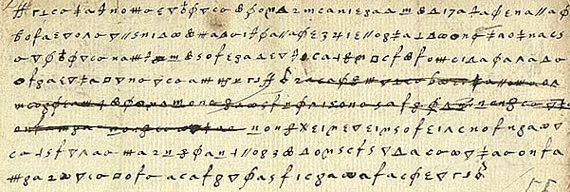
\includegraphics[width=\linewidth, height=1.5in, keepaspectratio]{../figure/encrypted_letter.jpg}
\caption{Snippet from encrypted communication between queen Mary and Sir
Babington}
\label{maryscottletterfig}
\end{marginfigure}

Mary used what's known as a \emph{substitution cipher} where each letter
is transformed into a different obscure symbol (see
\cref{maryscottletterfig}). At a first look, such a letter might seem
rather inscrutable- a meaningless sequence of strange symbols. However,
after some thought, one might recognize that these symbols \emph{repeat}
several times and moreover that different symbols repeat with different
frequencies. Now it doesn't take a large leap of faith to assume that
perhaps each symbol corresponds to a different letter and the more
frequent symbols correspond to letters that occur in the alphabet with
higher frequency. From this observation, there is a short gap to
completely breaking the cipher, which was in fact done by queen
Elisabeth's spies who used the decoded letters to learn of all the
co-conspirators and to convict queen Mary of treason, a crime for which
she was executed. Trusting in superficial security measures (such as
using ``inscrutable'' symbols) is a trap that users of cryptography have
been falling into again and again over the years. (As in many things,
this is the subject of a great XKCD cartoon, see \cref{XKCDnavajofig}.)


\begin{marginfigure}
\centering
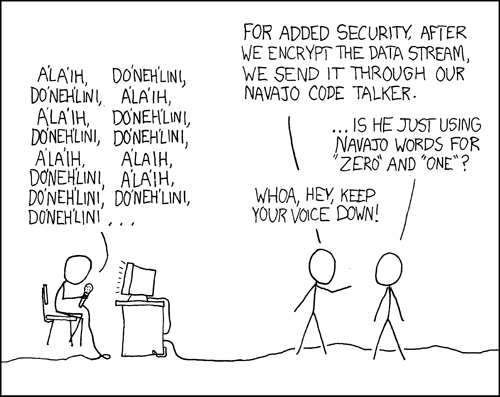
\includegraphics[width=\linewidth, height=1.5in, keepaspectratio]{../figure/code_talkers.png}
\caption{XKCD's take on the added security of using uncommon symbols}
\label{XKCDnavajofig}
\end{marginfigure}

The \href{https://en.wikipedia.org/wiki/Vigen\%C3\%A8re_cipher}{Vigenère
cipher} is named after Blaise de Vigenère who described it in a book in
1586 (though it was invented earlier by Bellaso). The idea is to use a
collection of substitution cyphers - if there are \(n\) different
ciphers then the first letter of the plaintext is encoded with the first
cipher, the second with the second cipher, the \(n^{th}\) with the
\(n^{th}\) cipher, and then the \(n+1^{st}\) letter is again encoded
with the first cipher. The key is usually a word or a phrase of \(n\)
letters, and the \(i^{th}\) substitution cipher is obtained by shifting
each letter \(k_i\) positions in the alphabet. This ``flattens'' the
frequencies and makes it much harder to do frequency analysis, which is
why this cipher was considered ``unbreakable'' for 300+ years and got
the nickname ``le chiffre indéchiffrable'' (``the unbreakable cipher'').
Nevertheless, Charles Babbage cracked the Vigenère cipher in 1854
(though he did not publish it). In 1863 Friedrich Kasiski broke the
cipher and published the result. The idea is that once you guess the
length of the cipher, you can reduce the task to breaking a simple
substitution cipher which can be done via frequency analysis (can you
see why?). Confederate generals used Vigenère regularly during the civil
war, and their messages were routinely cryptanalzed by Union officers.


\begin{marginfigure}
\centering
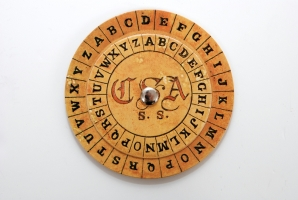
\includegraphics[width=\linewidth, height=1.5in, keepaspectratio]{../figure/confederate_cipher_disk.jpg}
\caption{Confederate Cipher Disk for implementing the Vigenère cipher}
\label{tmplabelfig}
\end{marginfigure}


\begin{marginfigure}
\centering
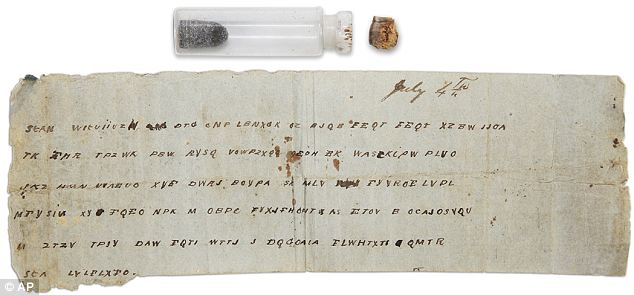
\includegraphics[width=\linewidth, height=1.5in, keepaspectratio]{../figure/confederate_message.jpg}
\caption{Confederate encryption of the message ``Gen'l Pemberton: You
can expect no help from this side of the river. Let Gen'l Johnston know,
if possible, when you can attack the same point on the enemy's lines.
Inform me also and I will endeavor to make a diversion. I have sent some
caps. I subjoin a despatch from General Johnston.''}
\label{tmplabelfig}
\end{marginfigure}

The \emph{Enigma} cipher was a mechanical cipher (looking like a
typewriter, see \cref{enigmafig}) where each letter typed would get
mapped into a different letter depending on the (rather complicated) key
and current state of the machine which had several rotors that rotated
at different paces. An identically wired machine at the other end could
be used to decrypt. Just as many ciphers in history, this has also been
believed by the Germans to be ``impossible to break'' and even quite
late in the war they refused to believe it was broken despite mounting
evidence to that effect. (In fact, some German generals refused to
believe it was broken even \emph{after} the war.) Breaking Enigma was an
heroic effort which was initiated by the Poles and then completed by the
British at Bletchley Park, with Alan Turing (of the Turing machines)
playing a key role. As part of this effort the Brits built arguably the
world's first large scale mechanical computation devices (though they
looked more similar to washing machines than to iPhones). They were also
helped along the way by some quirks and errors of the German operators.
For example, the fact that their messages ended with ``Heil Hitler''
turned out to be quite useful.


\begin{marginfigure}
\centering
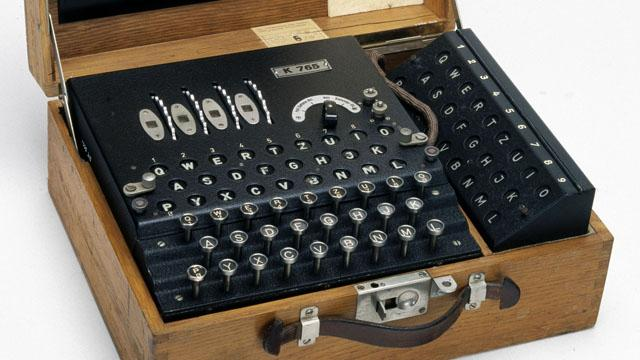
\includegraphics[width=\linewidth, height=1.5in, keepaspectratio]{../figure/enigma.jpg}
\caption{In the \emph{Enigma} mechanical cipher the secret key would be
the settings of the rotors and internal wires. As the operator types up
their message, the encrypted version appeared in the display area above,
and the internal state of the cipher was updated (and so typing the same
letter twice would generally result in two different letters output).
Decrypting follows the same process: if the sender and receiver are
using the same key then typing the ciphertext would result in the
plaintext appearing in the display.}
\label{enigmafig}
\end{marginfigure}

Here is one entertaining anecdote: the Enigma machine would never map a
letter to itself. In March 1941, Mavis Batey, a cryptanalyst at
Bletchley Park received a very long message that she tried to decrypt.
She then noticed a curious property--- the message did \emph{not}
contain the letter ``L''.\footnote{Here is a nice exercise: compute (up
  to an order of magnitude) the probability that a 50-letter long
  message composed of random letters will end up not containing the
  letter ``L''.} She realized that the probability that no ``L'''s
appeared in the message is too small for this to happen by chance. Hence
she surmised that the original message must have been composed
\emph{only} of L's. That is, it must have been the case that the
operator, perhaps to test the machine, have simply sent out a message
where he repeatedly pressed the letter ``L''. This observation helped
her decode the next message, which helped inform of a planned Italian
attack and secure a resounding British victory in what became known as
``the Battle of Cape Matapan''. Mavis also helped break another Enigma
machine. Using the information she provided, the Brits were able to feed
the Germans with the false information that the main allied invasion
would take place in Pas de Calais rather than on Normandy.

In the words of General Eisenhower, the intelligence from Bletchley park
was of ``priceless value''. It made a huge difference for the Allied war
effort, thereby shortening World War II and saving millions of lives.
See also \href{http://www.cix.co.uk/~klockstone/hinsley.htm}{this
interview with Sir Harry Hinsley}.

\section{Defining encryption}\label{Defining-encryption}

Many of the troubles that cryptosystem designers faced over history (and
still face!) can be attributed to not properly defining or understanding
what are the goals they want to achieve in the first place. Let us focus
on the setting of \emph{private key encryption}. (This is also known as
``symmetric encryption''; for thousands of years, ``private key
encryption'' was synonymous with encryption and only in the 1970's was
the concept of \emph{public key encryption} invented, see
\cref{publickeyencdef}.) A \emph{sender} (traditionally called
``Alice'') wants to send a message (known also as a \emph{plaintext})
\(x\in \{0,1\}^*\) to a \emph{receiver} (traditionally called ``Bob'').
They would like their message to be kept secret from an \emph{adversary}
who listens in or ``eavesdrops'' on the communication channel (and is
traditionally called ``Eve'').

Alice and Bob share a \emph{secret key} \(k \in \{0,1\}^*\). (While the
letter \(k\) is often used elsewhere in the book to denote a natural
number, in this chapter we use it to denote the string corresponding to
a secret key.) Alice uses the key \(k\) to ``scramble'' or
\emph{encrypt} the plaintext \(x\) into a \emph{ciphertext} \(y\), and
Bob uses the key \(k\) to ``unscramble'' or \emph{decrypt} the
ciphertext \(y\) back into the plaintext \(x\). This motivates the
following definition which attempts to capture what it means for an
encryption scheme to be \emph{valid} or ``make sense'', regardless of
whether or not it is \emph{secure}:

\hypertarget{encryptiondef}{}
\begin{definition}[Valid encryption scheme] \label[definition]{encryptiondef}

Let \(L:\N \rightarrow \N\) and \(C:\N \rightarrow \N\) be two functions
mapping natural numbers to natural numbers. A pair of polynomial-time
computable functions \((E,D)\) mapping strings to strings is a
\emph{valid private key encryption scheme} (or \emph{encryption scheme}
for short) with plaintext length function \(L(\cdot)\) and ciphertext
length function \(C(\cdot)\) if for every \(n\in \N\),
\(k\in \{0,1\}^n\) and \(x \in \{0,1\}^{L(n)}\), \(|E_k(x)|= C(n)\) and
\[
D(k,E(k,x))=x \;. \label{eqvalidenc}
\]

\end{definition}

We will often write the first input (i.e., the key) to the encryption
and decryption as a subscript and so can write \eqref{eqvalidenc} also
as \(D_k(E_k(x))=x\).


\begin{marginfigure}
\centering
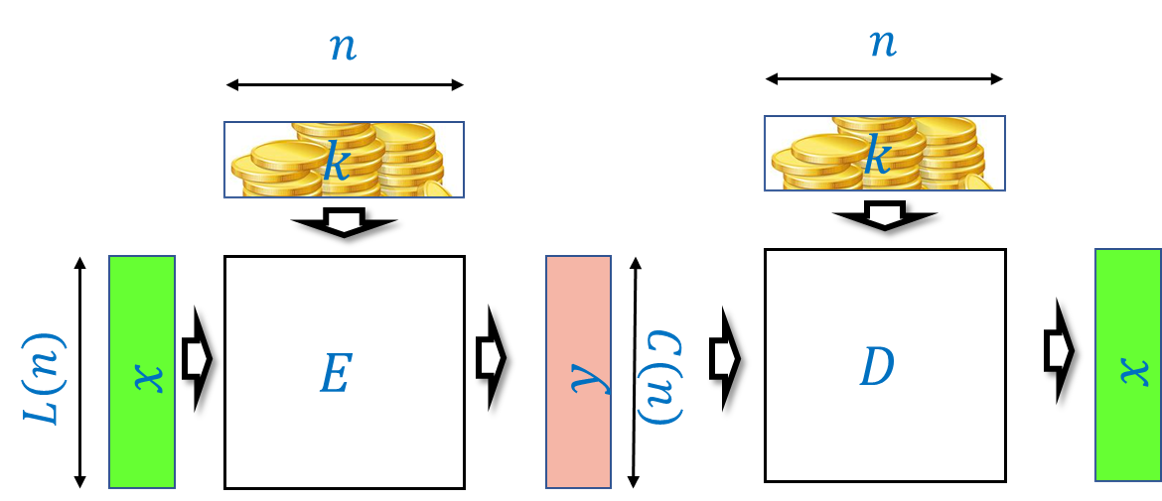
\includegraphics[width=\linewidth, height=1.5in, keepaspectratio]{../figure/encryptionvalid.png}
\caption{A private-key encryption scheme is a pair of algorithms \(E,D\)
such that for every key \(k\in \{0,1\}^n\) and plaintext
\(x\in \{0,1\}^{L(n)}\), \(y=E_k(x)\) is a ciphertext of length
\(C(n)\). The encryption scheme is \emph{valid} if for every such \(y\),
\(D_k(y)=x\). That is, the decryption of an encryption of \(x\) is
\(x\), as long as both encryption and decryption use the same key.}
\label{validencryption}
\end{marginfigure}

\hypertarget{lengthsciphertextplaintext}{}
\begin{solvedexercise}[Lengths of ciphertext and plaintext] \label[solvedexercise]{lengthsciphertextplaintext}

Prove that for every valid encryption scheme \((E,D)\) with functions
\(L,C\). \(C(n) \geq L(n)\) for every \(n\).

\end{solvedexercise}

\begin{solution} \label[solution]{For-every-fixed-key-k-in-}

For every fixed key \(k \in \{0,1\}^n\), the equation \eqref{eqvalidenc}
implies that the map \(y \mapsto D_k(y)\) inverts the map
\(x \mapsto E_k(x)\), which in particular means that the map
\(x \mapsto E_k(x)\) must be one to one. Hence its codomain must be at
least as large as its domain, and since its domain is \(\{0,1\}^{L(n)}\)
and its codomain is \(\{0,1\}^{C(n)}\) it follows that
\(C(n) \geq L(n)\).

\end{solution}

Since the ciphertext length is always at least the plaintext length (and
in most applications it is not much longer than that), we typically
focus on the plaintext length as the quantity to optimize in an
encryption scheme. The \emph{larger} \(L(n)\) is, the better the scheme,
since it means we need a shorter secret key to protect messages of the
same length.

\section{Defining security of
encryption}\label{Defining-security-of-encr}

\cref{encryptiondef} says nothing about the \emph{security} of \(E\) and
\(D\), and even allows the trivial encryption scheme that ignores the
key altogether and sets \(E_k(x)=x\) for every \(x\). Defining security
is not a trivial matter.

\begin{pause} \label[pause]{You-would-appreciate-the-}

You would appreciate the subtleties of defining security of encryption
more if at this point you take a five minute break from reading, and try
(possibly with a partner) to brainstorm on how you would mathematically
define the notion that an encryption scheme is \emph{secure}, in the
sense that it protects the secrecy of the plaintext \(x\).

\end{pause}

Throughout history, many attacks on cryptosystems were rooted in the
cryptosystem designers' reliance on ``security through obscurity''---
trusting that the fact their \emph{methods} are not known to their enemy
will protect them from being broken. This is a faulty assumption - if
you reuse a method again and again (even with a different key each time)
then eventually your adversaries will figure out what you are doing. And
if Alice and Bob meet frequently in a secure location to decide on a new
method, they might as well take the opportunity to exchange their
secrets. These considerations led Auguste Kerckhoffs in 1883 to state
the following principle:

\begin{quote}
\emph{A cryptosystem should be secure even if everything about the
system, except the key, is public knowledge.}\footnote{The actual quote
  is ``Il faut qu'il n'exige pas le secret, et qu'il puisse sans
  inconvénient tomber entre les mains de l'ennemi'' loosely translated
  as ``The system must not require secrecy and can be stolen by the
  enemy without causing trouble''. According to Steve Bellovin the NSA
  version is ``assume that the first copy of any device we make is
  shipped to the Kremlin''.}
\end{quote}

Why is it OK to assume the key is secret and not the algorithm? Because
we can always choose a fresh key. But of course that won't help us much
if our key is ``1234'' or ``passw0rd!''. In fact, if you use \emph{any}
deterministic algorithm to choose the key then eventually your adversary
will figure this out. Therefore for security we must choose the key at
\emph{random} and can restate Kerckhoffs's principle as follows:

\begin{quote}
\emph{There is no secrecy without randomness}
\end{quote}

This is such a crucial point that is worth repeating:

\hypertarget{securityrandomness}{}
\begin{bigidea} \label[bigidea]{securityrandomness}

There is no \emph{secrecy} without \emph{randomness}.

\end{bigidea}

At the heart of every cryptographic scheme there is a secret key, and
the secret key is always chosen at random. A corollary of that is that
to understand cryptography, you need to know probability theory.

\hypertarget{randomnessinlife}{}
\begin{remark}[Randomness in the real world] \label[remark]{randomnessinlife}

Choosing the secrets for cryptography requires generating randomness,
which is often done by measuring some ``unpredictable'' or ``high
entropy'' data, and then applying hash functions to the result to
``extract'' a uniformly random string. Great care must be taken in doing
this, and randomness generators often turn out to be the Achilles heel
of secure systems.

In 2006 a programmer removed a line of code from the procedure to
generate entropy in OpenSSL package distributed by Debian since it
caused a warning in some automatic verification code. As a result for
two years (until this was discovered) all the randomness generated by
this procedure used only the process ID as an ``unpredictable'' source.
This means that all communication done by users in that period is fairly
easily breakable (and in particular, if some entities recorded that
communication they could break it also retroactively). See
\href{http://www.xkcd.com/424/}{XKCD's take} on that incident.

In 2012 two separate teams of researchers scanned a large number of RSA
keys on the web and found out that about 4 percent of them are easy to
break. The main issue were devices such as routers, internet-connected
printers and such. These devices sometimes run variants of Linux- a
desktop operating system- but without a hard drive, mouse or keyboard,
they don't have access to many of the entropy sources that desktop have.
Coupled with some good old fashioned ignorance of cryptography and
software bugs, this led to many keys that are downright trivial to
break, see
\href{https://freedom-to-tinker.com/blog/nadiah/new-research-theres-no-need-panic-over-factorable-keys-just-mind-your-ps-and-qs/}{this
blog post} and \href{https://factorable.net/}{this web page} for more
details.

Since randomness is so crucial to security, breaking the procedure to
generate randomness can lead to a complete break of the system that uses
this randomness. Indeed, the Snowden documents, combined with
observations of Shumow and Ferguson,
\href{https://en.wikipedia.org/wiki/Dual_EC_DRBG}{strongly suggest} that
the NSA has deliberately inserted a \emph{trapdoor} in one of the
pseudorandom generators published by the National Institute of Standards
and Technologies (NIST). Fortunately, this generator wasn't widely
adapted but apparently the NSA did pay 10 million dollars to RSA
security so the latter would make this generator their default option in
their products.

\end{remark}

\section{Perfect secrecy}\label{Perfect-secrecy}

If you think about encryption scheme security for a while, you might
come up with the following principle for defining security: \emph{``An
encryption scheme is secure if it is not possible to recover the key
\(k\) from \(E_k(x)\)''}. However, a moment's thought shows that the key
is not really what we're trying to protect. After all, the whole point
of an encryption is to protect the confidentiality of the
\emph{plaintext} \(x\). So, we can try to define that \emph{``an
encryption scheme is secure if it is not possible to recover the
plaintext \(x\) from \(E_k(x)\)''}. Yet it is not clear what this means
either. Suppose that an encryption scheme reveals the first 10 bits of
the plaintext \(x\). It might still not be possible to recover \(x\)
completely, but on an intuitive level, this seems like it would be
extremely unwise to use such an encryption scheme in practice. Indeed,
often even \emph{partial information} about the plaintext is enough for
the adversary to achieve its goals.

The above thinking led Shannon in 1945 to formalize the notion of
\emph{perfect secrecy}, which is that an encryption reveals absolutely
nothing about the message. There are several equivalent ways to define
it, but perhaps the cleanest one is the following:

\hypertarget{perfectsecrecy}{}
\begin{definition}[Perfect secrecy] \label[definition]{perfectsecrecy}

A valid encryption scheme \((E,D)\) with plaintext length \(L(\cdot)\)
is \emph{perfectly secret} if for every \(n\in \N\) and plaintexts
\(x,x' \in \{0,1\}^{L(n)}\), the following two distributions \(Y\) and
\(Y'\) over \(\{0,1\}^*\) are identical:

\begin{itemize}
\item
  \(Y\) is obtained by sampling \(k\sim \{0,1\}^n\) and outputting
  \(E_k(x)\).
\item
  \(Y'\) is obtained by sampling \(k\sim \{0,1\}^n\) and outputting
  \(E_k(x')\).
\end{itemize}

\end{definition}

\begin{pause} \label[pause]{This-definition-might-tak}

This definition might take more than one reading to parse. Try to think
of how this condition would correspond to your intuitive notion of
``learning no information'' about \(x\) from observing \(E_k(x)\), and
to Shannon's quote in the beginning of this chapter.

In particular, suppose that you knew ahead of time that Alice sent
either an encryption of \(x\) or an encryption of \(x'\). Would you
learn anything new from observing the encryption of the message that
Alice actually sent? It may help you to look at \cref{perfectsecfig}.

\end{pause}


\begin{marginfigure}
\centering
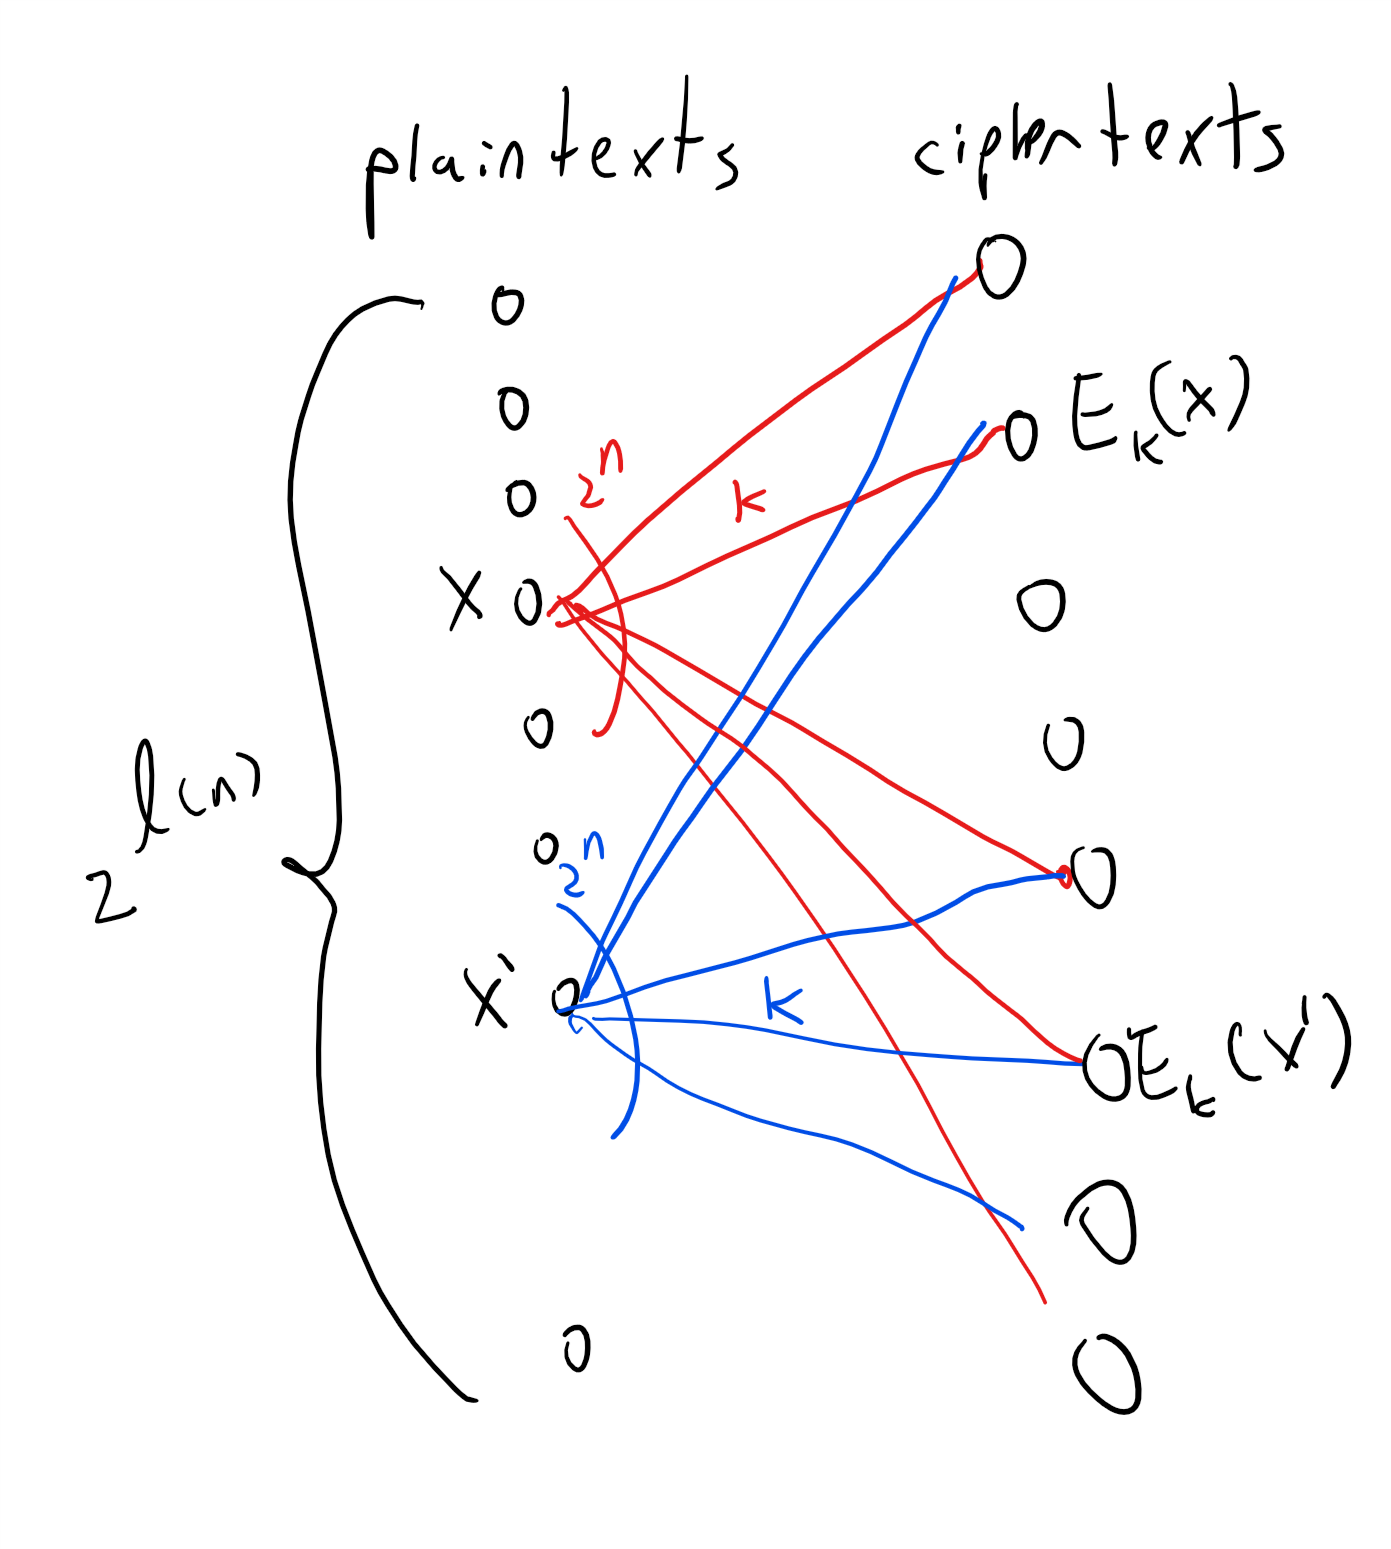
\includegraphics[width=\linewidth, height=1.5in, keepaspectratio]{../figure/perfectsecrecy.png}
\caption{For any key length \(n\), we can visualize an encryption scheme
\((E,D)\) as a graph with a vertex for every one of the \(2^{L(n)}\)
possible plaintexts and for every one of the ciphertexts in
\(\{0,1\}^*\) of the form \(E_k(x)\) for \(k\in \{0,1\}^n\) and
\(x\in \{0,1\}^{L(n)}\). For every plaintext \(x\) and key \(k\), we add
an edge labeled \(k\) between \(x\) and \(E_k(x)\). By the validity
condition, if we pick any fixed key \(k\), the map \(x \mapsto E_k(x)\)
must be one-to-one. The condition of perfect secrecy simply corresponds
to requiring that every two plaintexts \(x\) and \(x'\) have exactly the
same set of neighbors (or multi-set, if there are parallel edges).}
\label{perfectsecfig}
\end{marginfigure}

\subsection{Example: Perfect secrecy in the
battlefield}\label{Example-Perfect-secrecy-i}

To understand \cref{perfectsecrecy}, suppose that Alice sends only one
of two possible messages: ``attack'' or ``retreat'', which we denote by
\(x_0\) and \(x_1\) respectively, and that she sends each one of those
messages with probability \(1/2\). Let us put ourselves in the shoes of
\emph{Eve}, the eavesdropping adversary. A priori we would have guessed
that Alice sent either \(x_0\) or \(x_1\) with probability \(1/2\). Now
we observe \(y=E_k(x_i)\) where \(k\) is a uniformly chosen key in
\(\{0,1\}^n\). How does this new information cause us to update our
beliefs on whether Alice sent the plaintext \(x_0\) or the plaintext
\(x_1\)?

\begin{pause} \label[pause]{Before-reading-the-next-p}

Before reading the next paragraph, you might want to try the analysis
yourself. You may find it useful to look at the
\href{https://en.wikipedia.org/wiki/Bayesian_inference}{Wikipedia entry
on Bayesian Inference} or
\href{https://ocw.mit.edu/courses/mathematics/18-05-introduction-to-probability-and-statistics-spring-2014/readings/MIT18_05S14_Reading11.pdf}{these
MIT lecture notes}.

\end{pause}

Let us define \(p_0(y)\) to be the probability (taken over
\(k\sim \{0,1\}^n\)) that \(y=E_k(x_0)\) and similarly \(p_1(y)\) to be
\(\Pr_{k \sim \{0,1\}^n}[y=E_k(x_1)]\). Note that, since Alice chooses
the message to send at random, our a priori probability for observing
\(y\) is \(\tfrac{1}{2}p_0(y) + \tfrac{1}{2}p_1(y)\). However, as per
\cref{perfectsecrecy}, the perfect secrecy condition guarantees that
\(p_0(y)=p_1(y)\)! Let us denote the number \(p_0(y)=p_1(y)\) by \(p\).
By the formula for conditional probability, the probability that Alice
sent the message \(x_0\) conditioned on our observation \(y\) is simply
\[
\Pr[i=0 | y=E_k(x_i)] = \frac{\Pr[i=0 \wedge y = E_k(x_i)]}{\Pr[y = E_k(x)]} \;. \label{bayeseq}
\]

(The equation \eqref{bayeseq} is a special case of \emph{Bayes' rule}
which, although a simple restatement of the formula for conditional
probability, is an extremely important and widely used tool in
statistics and data analysis.)

Since the probability that \(i=0\) and \(y\) is the ciphertext
\(E_k(0)\) is equal to \(\tfrac{1}{2}\cdot p_0(y)\), and the a priori
probability of observing \(y\) is
\(\tfrac{1}{2}p_0(y) + \tfrac{1}{2}p_1(y)\), we can rewrite
\eqref{bayeseq} as \[
\Pr[i=0 | y=E_k(x_i)] = \frac{\tfrac{1}{2}p_0(y)}{\tfrac{1}{2}p_0(y)+\tfrac{1}{2}p_1(y)}  =  \frac{p}{p +p}  = \frac{1}{2}
\] using the fact that \(p_0(y)=p_1(y)=p\). This means that observing
the ciphertext \(y\) did not help us at all! We still would not be able
to guess whether Alice sent ``attack'' or ``retreat'' with better than
50/50 odds!

This example can be vastly generalized to show that perfect secrecy is
indeed ``perfect'' in the sense that observing a ciphertext gives Eve
\emph{no additional information} about the plaintext beyond her a priori
knowledge.

\subsection{Constructing perfectly secret
encryption}\label{Constructing-perfectly-se}

\emph{Perfect secrecy} is an extremely strong condition, and implies
that an eavesdropper does not learn \emph{any} information from
observing the ciphertext. You might think that an encryption scheme
satisfying such a strong condition will be impossible, or at least
extremely complicated, to achieve. However it turns out we can in fact
obtain perfectly secret encryption scheme fairly easily. Such a scheme
for two-bit messages is illustrated in \cref{onetimepadtwofig}


\begin{marginfigure}
\centering
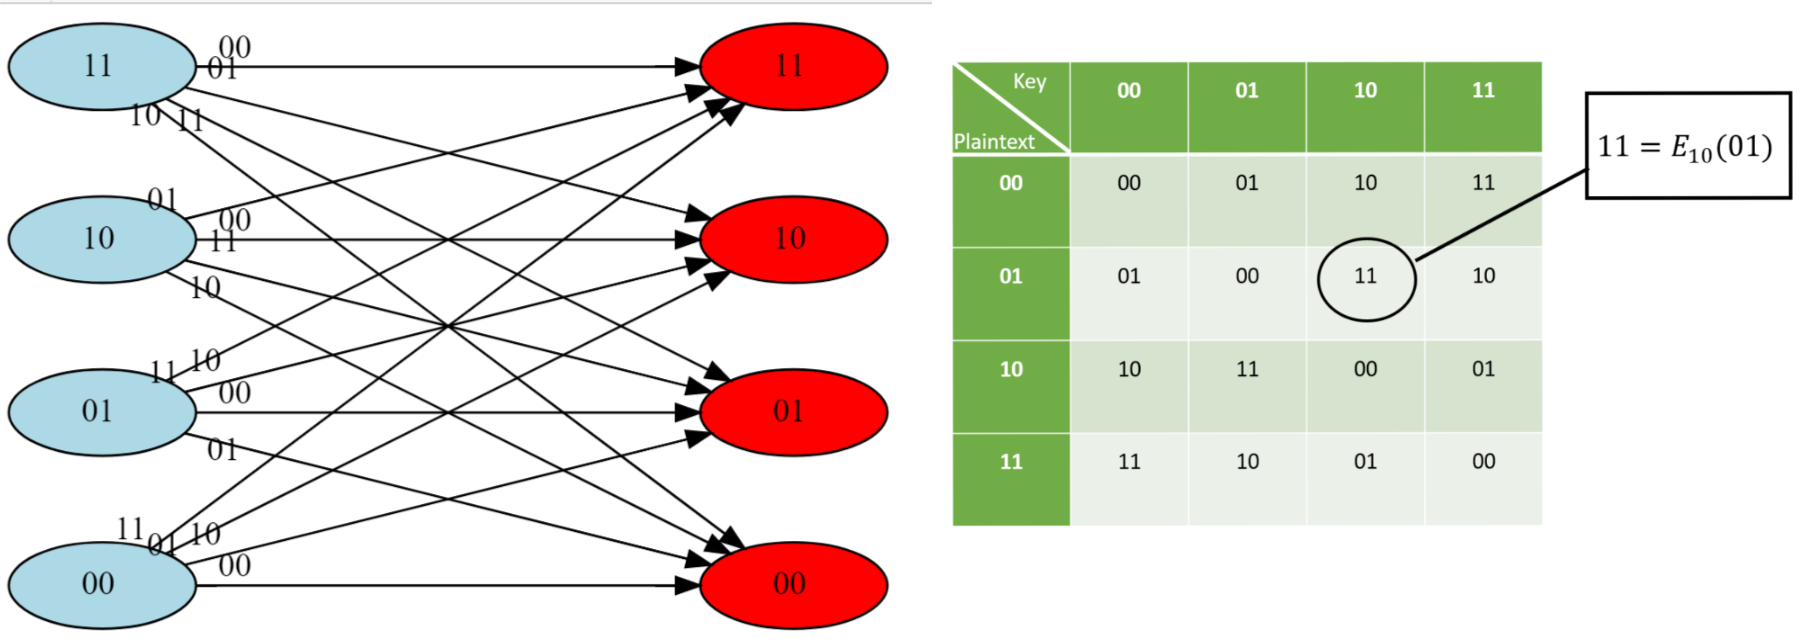
\includegraphics[width=\linewidth, height=1.5in, keepaspectratio]{../figure/onetimepadtwobits.png}
\caption{A perfectly secret encryption scheme for two-bit keys and
messages. The blue vertices represent plaintexts and the red vertices
represent ciphertexts, each edge mapping a plaintext \(x\) to a
ciphertext \(y=E_k(x)\) is labeled with the corresponding key \(k\).
Since there are four possible keys, the degree of the graph is four and
it is in fact a complete bipartite graph. The encryption scheme is valid
in the sense that for every \(k\in \{0,1\}^2\), the map
\(x \mapsto E_k(x)\) is one-to-one, which in other words means that the
set of edges labeled with \(k\) is a \emph{matching}.}
\label{onetimepadtwofig}
\end{marginfigure}

In fact, this can be generalized to any number of bits:

\hypertarget{onetimepad}{}
\begin{theorem}[One Time Pad (Vernam 1917, Shannon 1949)] \label[theorem]{onetimepad}

There is a perfectly secret valid encryption scheme \((E,D)\) with
\(L(n)=C(n)=n\).

\end{theorem}

\begin{proofidea} \label[proofidea]{Our-scheme-is-the-one-tim}

Our scheme is the
\href{https://en.wikipedia.org/wiki/One-time_pad}{one-time pad} also
known as the ``Vernam Cipher'', see \cref{onetimepadfig}. The encryption
is exceedingly simple: to encrypt a message \(x\in \{0,1\}^n\) with a
key \(k \in \{0,1\}^n\) we simply output \(x \oplus k\) where \(\oplus\)
is the bitwise XOR operation that outputs the string corresponding to
XORing each coordinate of \(x\) and \(k\).

\end{proofidea}

\begin{proof}[Proof of \cref{onetimepad}] \label[proof]{For-two-binary-strings-a-}

For two binary strings \(a\) and \(b\) of the same length \(n\), we
define \(a \oplus b\) to be the string \(c \in \{0,1\}^n\) such that
\(c_i = a_i + b_i \mod 2\) for every \(i\in [n]\). The encryption scheme
\((E,D)\) is defined as follows: \(E_k(x) = x\oplus k\) and
\(D_k(y)= y \oplus k\). By the associative law of addition (which works
also modulo two),
\(D_k(E_k(x))=(x\oplus k) \oplus k = x \oplus (k \oplus k) = x \oplus 0^n = x\),
using the fact that for every bit \(\sigma \in \{0,1\}\),
\(\sigma + \sigma \mod 2 = 0\) and \(\sigma + 0 = \sigma \mod 2\). Hence
\((E,D)\) form a valid encryption.

To analyze the perfect secrecy property, we claim that for every
\(x\in \{0,1\}^n\), the distribution \(Y_x=E_k(x)\) where
\(k \sim \{0,1\}^n\) is simply the uniform distribution over
\(\{0,1\}^n\), and hence in particular the distributions \(Y_{x}\) and
\(Y_{x'}\) are identical for every \(x,x' \in \{0,1\}^n\). Indeed, for
every particular \(y\in \{0,1\}^n\), the value \(y\) is output by
\(Y_x\) if and only if \(y = x \oplus k\) which holds if and only if
\(k= x \oplus y\). Since \(k\) is chosen uniformly at random in
\(\{0,1\}^n\), the probability that \(k\) happens to equal
\(x \oplus y\) is exactly \(2^{-n}\), which means that every string
\(y\) is output by \(Y_x\) with probability \(2^{-n}\).

\end{proof}


\begin{marginfigure}
\centering
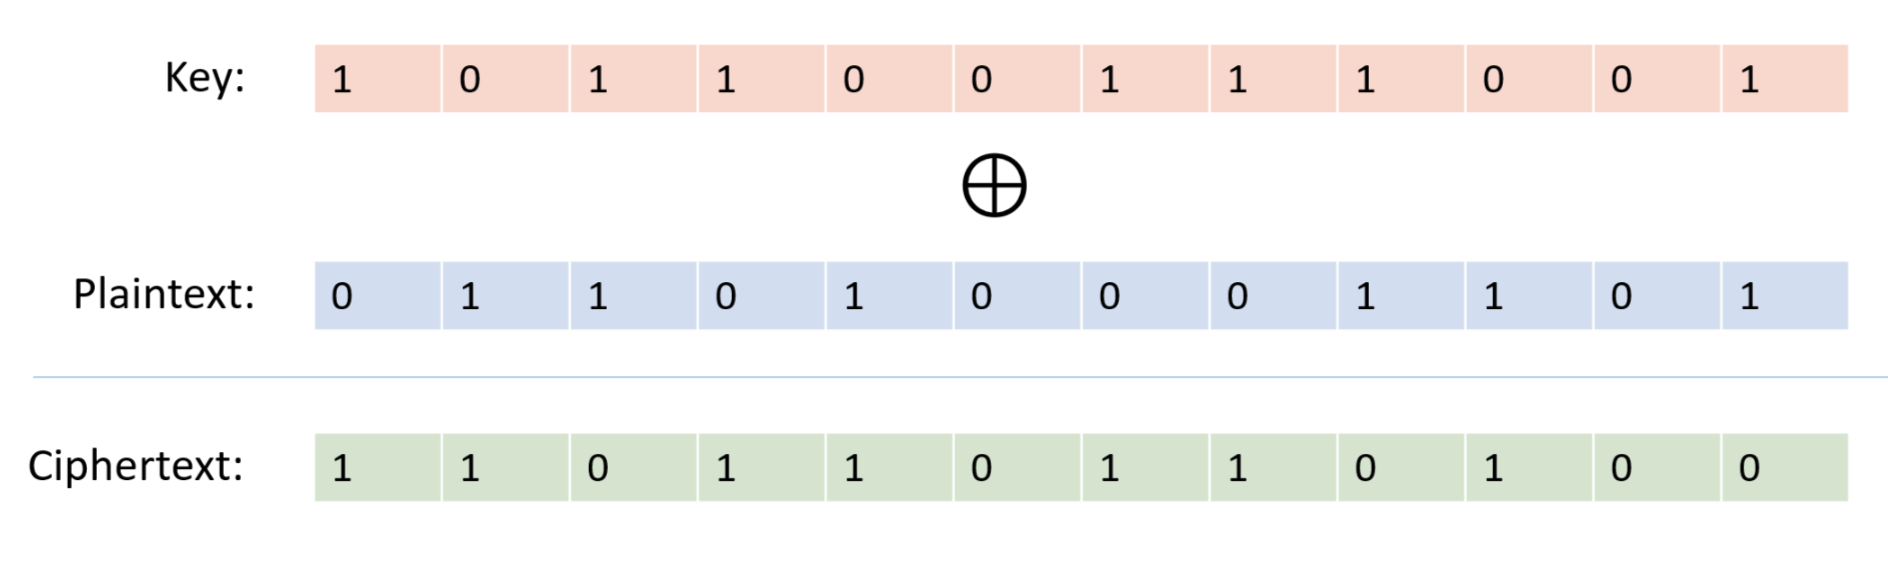
\includegraphics[width=\linewidth, height=1.5in, keepaspectratio]{../figure/onetimepad.png}
\caption{In the \emph{one time pad} encryption scheme we encrypt a
plaintext \(x\in \{0,1\}^n\) with a key \(k\in \{0,1\}^n\) by the
ciphertext \(x \oplus k\) where \(\oplus\) denotes the bitwise XOR
operation.}
\label{onetimepadfig}
\end{marginfigure}

\begin{pause} \label[pause]{The-argument-above-is-qui}

The argument above is quite simple but is worth reading again. To
understand why the one-time pad is perfectly secret, it is useful to
envision it as a bipartite graph as we've done in
\cref{onetimepadtwofig}. (In fact the encryption scheme of
\cref{onetimepadtwofig} is precisely the one-time pad for \(n=2\).) For
every \(n\), the one-time pad encryption scheme corresponds to a
bipartite graph with \(2^n\) vertices on the ``left side'' corresponding
to the plaintexts in \(\{0,1\}^n\) and \(2^n\) vertices on the ``right
side'' corresponding to the ciphertexts \(\{0,1\}^n\). For every
\(x\in \{0,1\}^n\) and \(k\in \{0,1\}^n\), we connect \(x\) to the
vertex \(y=E_k(x)\) with an edge that we label with \(k\). One can see
that this is the complete bipartite graph, where every vertex on the
left is connected to \emph{all} vertices on the right. In particular
this means that for every left vertex \(x\), the distribution on the
ciphertexts obtained by taking a random \(k\in \{0,1\}^n\) and going to
the neighbor of \(x\) on the edge labeled \(k\) is the uniform
distribution over \(\{0,1\}^n\). This ensures the perfect secrecy
condition.

\end{pause}

\section{Necessity of long keys}\label{Necessity-of-long-keys}

So, does \cref{onetimepad} give the final word on cryptography, and
means that we can all communicate with perfect secrecy and live happily
ever after? No it doesn't. While the one-time pad is efficient, and
gives perfect secrecy, it has one glaring disadvantage: to communicate
\(n\) bits you need to store a key of length \(n\). In contrast,
practically used cryptosystems such as AES-128 have a short key of
\(128\) bits (i.e., \(16\) bytes) that can be used to protect terabytes
or more of communication! Imagine that we all needed to use the one time
pad. If that was the case, then if you had to communicate with \(m\)
people, you would have to maintain (securely!) \(m\) huge files that are
each as long as the length of the maximum total communication you expect
with that person. Imagine that every time you opened an account with
Amazon, Google, or any other service, they would need to send you in the
mail (ideally with a secure courier) a DVD full of random numbers, and
every time you suspected a virus, you'd need to ask all these services
for a fresh DVD. This doesn't sound so appealing.

This is not just a theoretical issue. The Soviets have used the one-time
pad for their confidential communication since before the 1940's. In
fact, even before Shannon's work, the U.S. intelligence already knew in
1941 that the one-time pad is in principle ``unbreakable'' (see page 32
in the \href{http://nsarchive.gwu.edu/NSAEBB/NSAEBB278/01.PDF}{Venona
document}). However, it turned out that the hassle of manufacturing so
many keys for all the communication took its toll on the Soviets and
they ended up reusing the same keys for more than one message. They did
try to use them for completely different receivers in the (false) hope
that this wouldn't be detected. The
\href{https://en.wikipedia.org/wiki/Venona_project}{Venona Project} of
the U.S. Army was founded in February 1943 by Gene Grabeel (see
\cref{genegrabeelfig}), a former home economics teacher from Madison
Heights, Virgnia and Lt. Leonard Zubko. In October 1943, they had their
breakthrough when it was discovered that the Russians were reusing their
keys. In the 37 years of its existence, the project has resulted in a
treasure chest of intelligence, exposing hundreds of KGB agents and
Russian spies in the U.S. and other countries, including Julius
Rosenberg, Harry Gold, Klaus Fuchs, Alger Hiss, Harry Dexter White and
many others.


\begin{marginfigure}
\centering
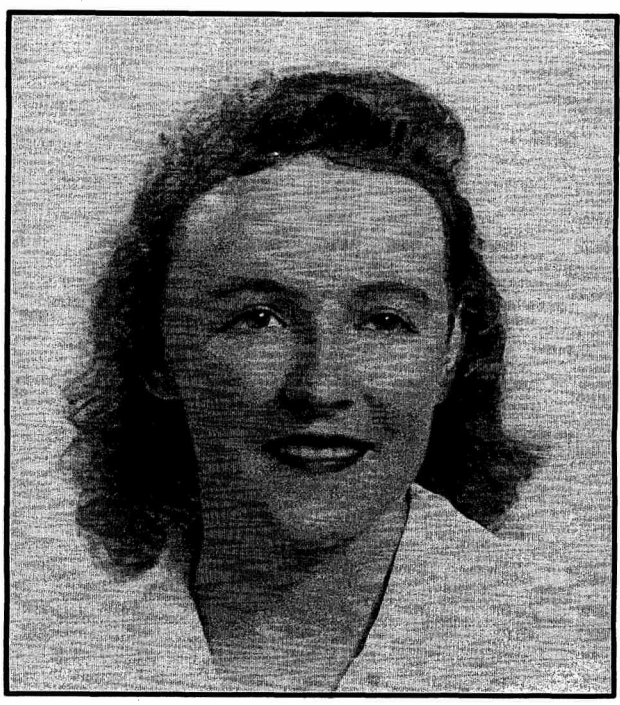
\includegraphics[width=\linewidth, height=1.5in, keepaspectratio]{../figure/genevenona.png}
\caption{Gene Grabeel, who founded the U.S. Russian SigInt program on 1
Feb 1943. Photo taken in 1942, see Page 7 in the Venona historical
study.}
\label{genegrabeelfig}
\end{marginfigure}


\begin{marginfigure}
\centering
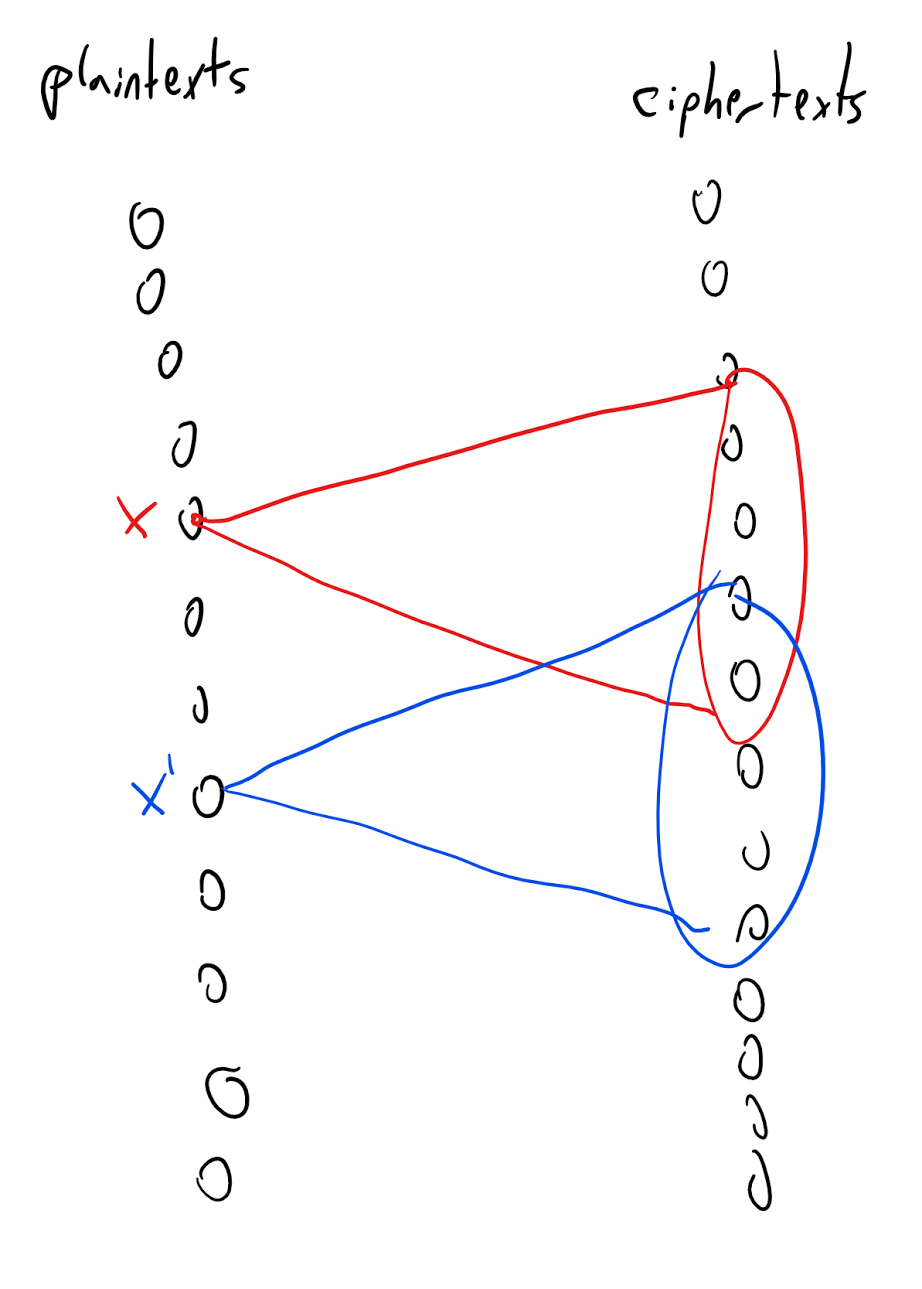
\includegraphics[width=\linewidth, height=1.5in, keepaspectratio]{../figure/longkeygraph.png}
\caption{An encryption scheme where the number of keys is smaller than
the number of plaintexts corresponds to a bipartite graph where the
degree is smaller than the number of vertices on the left side. Together
with the validity condition this implies that there will be two left
vertices \(x,x'\) with non-identical neighborhoods, and hence the scheme
does \emph{not} satisfy perfect secrecy.}
\label{longkeygraphfig}
\end{marginfigure}

Unfortunately it turns out that that such long keys are \emph{necessary}
for perfect secrecy:

\hypertarget{longkeysthm}{}
\begin{theorem}[Perfect secrecy requires long keys] \label[theorem]{longkeysthm}

For every perfectly secret encryption scheme \((E,D)\) the length
function \(L\) satisfies \(L(n) \leq n\).

\end{theorem}

\begin{proofidea} \label[proofidea]{The-idea-behind-the-proof}

The idea behind the proof is illustrated in \cref{longkeygraphfig}. We
define a graph between the plaintexts and ciphertexts, where we put an
edge between plaintext \(x\) and ciphertext \(y\) if there is some key
\(k\) such that \(y=E_k(x)\). The \emph{degree} of this graph is at most
the number of potential keys. The fact that the degree is smaller than
the number of plaintexts (and hence of ciphertexts) implies that there
would be two plaintexts \(x\) and \(x'\) with different sets of
neighbors, and hence the distribution of a ciphertext corresponding to
\(x\) (with a random key) will not be identical to the distribution of a
ciphertext corresponding to \(x'\).

\end{proofidea}

\begin{proof}[Proof of \cref{longkeysthm}] \label[proof]{Let-ED-be-a-valid-encrypt}

Let \(E,D\) be a valid encryption scheme with messages of length \(L\)
and key of length \(n<L\). We will show that \((E,D)\) is not perfectly
secret by providing two plaintexts \(x_0,x_1 \in \{0,1\}^L\) such that
the distributions \(Y_{x_0}\) and \(Y_{x_1}\) are not identical, where
\(Y_x\) is the distribution obtained by picking \(k \sim \{0,1\}^n\) and
outputting \(E_k(x)\).

We choose \(x_0 = 0^L\). Let \(S_0 \subseteq \{0,1\}^*\) be the set of
all ciphertexts that have nonzero probability of being output in
\(Y_{x_0}\). That is,
\(S_0=\{ y \;|\; \exists_{k\in \{0,1\}^n} y=E_k(x_0) \}\). Since there
are only \(2^n\) keys, we know that \(|S_0| \leq 2^n\).

We will show the following claim:

\textbf{Claim I:} There exists some \(x_1 \in \{0,1\}^L\) and
\(k\in \{0,1\}^n\) such that \(E_k(x_1) \not\in S_0\).

Claim I implies that the string \(E_k(x_1)\) has positive probability of
being output by \(Y_{x_1}\) and zero probability of being output by
\(Y_{x_0}\) and hence in particular \(Y_{x_0}\) and \(Y_{x_1}\) are not
identical. To prove Claim I, just choose a fixed \(k\in \{0,1\}^n\). By
the validity condition, the map \(x \mapsto E_k(x)\) is a one to one map
of \(\{0,1\}^L\) to \(\{0,1\}^*\) and hence in particular the
\emph{image} of this map which is the set
\(I_k = \{ y \;|\; \exists_{x\in \{0,1\}^L} y=E_k(x) \}\) has size at
least (in fact exactly) \(2^L\). Since \(|S_0| \leq 2^n < 2^L\), this
means that \(|I_k|>|S_0|\) and so in particular there exists some string
\(y\) in \(I_k \setminus S_0\). But by the definition of \(I_k\) this
means that there is some \(x\in \{0,1\}^L\) such that
\(E_k(x) \not\in S_0\) which concludes the proof of Claim I and hence of
\cref{longkeysthm}.

\end{proof}

\section{Computational secrecy}\label{Computational-secrecy}

To sum up the previous episodes, we now know that:

\begin{itemize}
\tightlist
\item
  It is possible to obtain a perfectly secret encryption scheme with key
  length the same as the plaintext.
\end{itemize}

and

\begin{itemize}
\tightlist
\item
  It is not possible to obtain such a scheme with key that is even a
  single bit shorter than the plaintext.
\end{itemize}

How does this mesh with the fact that, as we've already seen, people
routinely use cryptosystems with a 16 byte (i.e., 128 bit) key but many
terabytes of plaintext? The proof of \cref{longkeysthm} does give in
fact a way to break all these cryptosystems, but an examination of this
proof shows that it only yields an algorithm with time \emph{exponential
in the length of the key}. This motivates the following relaxation of
perfect secrecy to a condition known as \emph{``computational
secrecy''}. Intuitively, an encryption scheme is computationally secret
if no polynomial time algorithm can break it. The formal definition is
below:

\hypertarget{compsecdef}{}
\begin{definition}[Computational secrecy] \label[definition]{compsecdef}

Let \((E,D)\) be a valid encryption scheme where for keys of length
\(n\), the plaintexts are of length \(L(n)\) and the ciphertexts are of
length \(m(n)\). We say that \((E,D)\) is \emph{computationally secret}
if for every polynomial \(p:\N \rightarrow \N\), and large enough \(n\),
if \(P\) is an \(m(n)\)-input and single output NAND-CIRC program of at
most \(p(n)\) lines, and \(x_0,x_1 \in \{0,1\}^{L(n)}\) then

\[
\left| \E_{k \sim \{0,1\}^n} [P(E_k(x_0))] -   \E_{k \sim \{0,1\}^n} [P(E_k(x_1))] \right| < \tfrac{1}{p(n)} \label{eqindist}
\]

\end{definition}

\begin{pause} \label[pause]{crefcompsecdef-requires-a}

\cref{compsecdef} requires a second or third read and some practice to
truly understand. One excellent exercise to make sure you follow it is
to see that if we allow \(P\) to be an \emph{arbitrary} function mapping
\(\{0,1\}^{m(n)}\) to \(\{0,1\}\), and we replace the condition in
\eqref{eqindist} that the lefthand side is smaller than
\(\tfrac{1}{p(L(n))}\) with the condition that it is equal to \(0\) then
we get the perfect secrecy condition of \cref{perfectsecrecy}. Indeed if
the distributions \(E_k(x_0)\) and \(E_k(x_1)\) are identical then
applying any function \(P\) to them we get the same expectation. On the
other hand, if the two distributions above give a different probability
for some element \(y^*\in \{0,1\}^{m(n)}\), then the function \(P(y)\)
that outputs \(1\) iff \(y=y^*\) will have a different expectation under
the former distribution than under the latter.

\end{pause}

\cref{compsecdef} raises two natural questions:

\begin{itemize}
\item
  Is it strong enough to ensure that a computationally secret encryption
  scheme protects the secrecy of messages that are encrypted with it?
\item
  It is weak enough that, unlike perfect secrecy, it is possible to
  obtain a computationally secret encryption scheme where the key is
  much smaller than the message?
\end{itemize}

To the best of our knowledge, the answer to both questions is
\emph{Yes}.

\hypertarget{computationcrypto}{}
\begin{bigidea} \label[bigidea]{computationcrypto}

\emph{Computational hardness} is necessary and sufficient for a great
many cryptographic constructions, and in particular for encryption
schemes with keys shorter than the message.

\end{bigidea}

Regarding the first question, it is not hard to show that if, for
example, Alice uses a computationally secret encryption algorithm to
encrypt either ``attack'' or ``retreat'' (each chosen with probability
\(1/2\)), then as long as she's restricted to polynomial-time
algorithms, an adversary Eve will not be able to guess the message with
probability better than, say, \(0.51\), even after observing its
encrypted form. (We omit the proof, but it is an excellent exercise for
you to work it out on your own.)

To answer the second question we will show that under the same
assumption we used for derandomizing \(\mathbf{BPP}\), we can obtain a
computationally secret cryptosystem where the key is almost
\emph{exponentially} smaller than the plaintext.

\subsection{Stream ciphers or the ``derandomized one-time
pad''}\label{Stream-ciphers-or-the-der}

It turns out that if pseudorandom generators exist as in the optimal PRG
conjecture, then there exists a computationally secret encryption scheme
with keys that are much shorter than the plaintext. The construction
below is known as a
\href{https://en.wikipedia.org/wiki/Stream_cipher}{stream cipher},
though perhaps a better name is the ``derandomized one-time pad''. It is
widely used in practice with keys on the order of a few tens or hundreds
of bits protecting many terabytes or even petabytes of communication.


\begin{marginfigure}
\centering
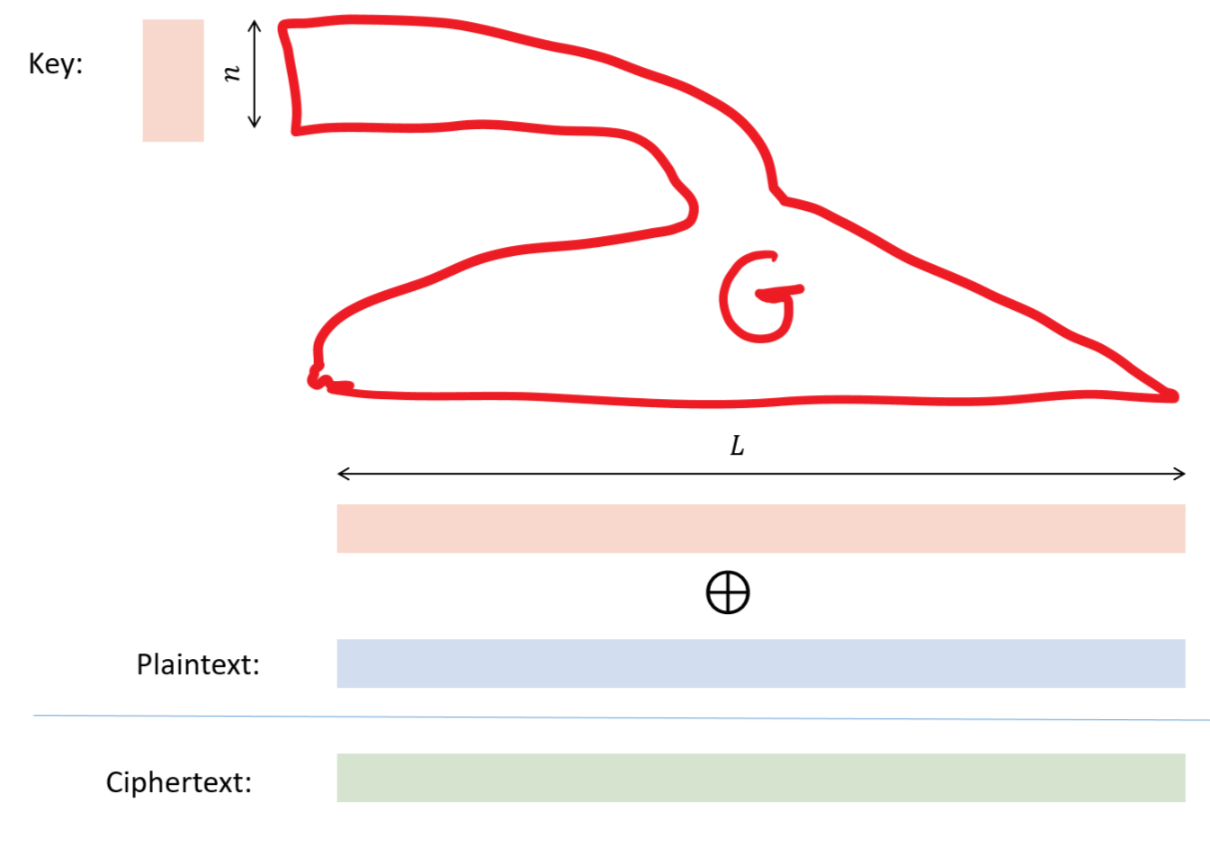
\includegraphics[width=\linewidth, height=1.5in, keepaspectratio]{../figure/derandonetimepad.png}
\caption{In a \emph{stream cipher} or ``derandomized one-time pad'' we
use a pseudorandom generator \(G:\{0,1\}^n \rightarrow \{0,1\}^L\) to
obtain an encryption scheme with a key length of \(n\) and plaintexts of
length \(L\). We encrypt the plaintext \(x\in \{0,1\}^L\) with key
\(k\in \{0,1\}^n\) by the ciphertext \(x \oplus G(k)\).}
\label{derandonetimepadfig}
\end{marginfigure}

We start by recalling the notion of a \emph{pseudorandom generator}, as
defined in \cref{prgdef}. For this chapter, we will fix a special case
of the definition:

\hypertarget{cryptoprg}{}
\begin{definition}[Cryptographic pseudorandom generator] \label[definition]{cryptoprg}

Let \(L:\N \rightarrow \N\) be some function. A \emph{cryptographic
pseudorandom generator} with stretch \(L(\cdot)\) is a polynomial-time
computable function \(G:\{0,1\}^* \rightarrow \{0,1\}^*\) such that:

\begin{itemize}
\item
  For every \(n\in \N\) and \(s\in \{0,1\}^n\), \(|G(s)|=L(n)\).
\item
  For every polynomial \(p:\N \rightarrow \N\) and \(n\) large enough,
  if \(C\) is a circuit of \(L(n)\) inputs, one output, and at most
  \(p(n)\) gates then \[
  \left| \Pr_{s\sim \{0,1\}^\ell}[C(G(s))=1] - \Pr_{r \sim \{0,1\}^m}[C(r)=1] \right| < \frac{1}{p(n)} \;.
  \]
\end{itemize}

\end{definition}

In this chapter we will call a cryptographic pseudorandom generator
simply a \emph{pseudorandom generator} or PRG for short. The optimal PRF
conjecture of \cref{optimalprgconj} implies that there is a pseudorandom
generator that can ``fool'' circuits of \emph{exponential size} and
where the gap in probabilities is at most one over an exponential
quantity. Since exponential grow faster than every polynomial, the
optimal PRG conjecture implies the following:

\begin{quote}
\textbf{The crypto PRG conjecture:} For every \(a \in \N\), there is a
cryptographic pseudorandom generator with \(L(n)=n^a\).
\end{quote}

The crypto PRG conjecture is a weaker conjecture than the optimal PRG
conjecture, but it too (as we will see) is still stronger than the
conjecture that \(\mathbf{P} \neq \mathbf{NP}\).

\hypertarget{PRGtoENC}{}
\begin{theorem}[Derandomized one-time pad] \label[theorem]{PRGtoENC}

Suppose that the crypto PRG conjecture is true. Then for every constant
\(a\in \N\) there is a computationally secret encryption scheme
\((E,D)\) with plaintext length \(L(n)\) at least \(n^a\).

\end{theorem}

\begin{proofidea} \label[proofidea]{The-proof-is-illustrated-}

The proof is illustrated in \cref{derandonetimepadfig}. We simply take
the one-time pad on \(L\) bit plaintexts, but replace the key with
\(G(k)\) where \(k\) is a string in \(\{0,1\}^n\) and
\(G:\{0,1\}^n \rightarrow \{0,1\}^L\) is a pseudorandom generator. Since
the one time pad cannot be broken, an adversary that breaks the
derandomized one-time pad can be used to distinguish between the output
of the pseudorandom generator and the uniform distribution.

\end{proofidea}

\begin{proof}[Proof of \cref{PRGtoENC}] \label[proof]{Let-Gn-rightarrow-L-for-L}

Let \(G:\{0,1\}^n \rightarrow \{0,1\}^L\) for \(L = n^a\) be the
restriction to input length \(n\) of the pseudorandom generator \(G\)
whose existence we are guaranteed from the crypto PRG conjecture. We now
define our encryption scheme as follows: given key \(k\in \{0,1\}^n\)
and plaintext \(x\in \{0,1\}^L\), the encryption \(E_k(x)\) is simply
\(x \oplus G(k)\). To decrypt a string \(y \in \{0,1\}^m\) we output
\(y \oplus G(k)\). This is a valid encryption since \(G\) is computable
in polynomial time and
\((x \oplus G(k)) \oplus G(k) = x \oplus (G(k) \oplus G(k))=x\) for
every \(x\in \{0,1\}^L\).

Computational secrecy follows from the condition of a pseudorandom
generator. Suppose, towards a contradiction, that there is a polynomial
\(p\), NAND-CIRC program \(Q\) of at most \(p(L)\) lines and
\(x,x' \in \{0,1\}^{L(n)}\) such that \[
\left| \E_{k \sim \{0,1\}^n}[ Q(E_k(x))] - \E_{k \sim \{0,1\}^n}[Q(E_k(x'))] \right| > \tfrac{1}{p(L)} \;.
\] (We use here the simple fact that for a \(\{0,1\}\)-valued random
variable \(X\), \(\Pr[X=1]=\E[X]\).)

By the definition of our encryption scheme, this means that \[
\left| \E_{k \sim \{0,1\}^n}[ Q(G(k) \oplus x)] - \E_{k \sim \{0,1\}^n}[Q(G(k) \oplus x')] \right| > \tfrac{1}{p(L)} \;. \label{eqprgsecone}
\]

Now since (as we saw in the security analysis of the one-time pad), for
every strings \(x,x'\in \{0,1\}^L\), the distribution \(r \oplus x\) and
\(r \oplus x'\) are identical, where \(r\sim \{0,1\}^L\). Hence \[
\E_{r \sim \{0,1\}^L} [ Q(r \oplus x)] =  \E_{r \sim \{0,1\}^L} [ Q(r \oplus x')]  \;.  \label{eqprgsectwo}
\] By plugging \eqref{eqprgsectwo} into \eqref{eqprgsecone} we can
derive that \[
\left| \E_{k \sim \{0,1\}^n}[ Q(G(k) \oplus x)] - \E_{r \sim \{0,1\}^L} [ Q(r \oplus x)] +  \E_{r \sim \{0,1\}^L} [ Q(r \oplus x')]  -  \E_{k \sim \{0,1\}^n}[Q(G(k) \oplus x')] \right| > \tfrac{1}{p(L)} \;. \label{eqprgsethree}
\] (Please make sure that you can see why this is true.)

Now we can use the \emph{triangle inequality} that
\(|A+B| \leq |A|+|B|\) for every two numbers \(A,B\), applying it for
\(A= \E_{k \sim \{0,1\}^n}[ Q(G(k) \oplus x)] - \E_{r \sim \{0,1\}^L} [ Q(r \oplus x)]\)
and
\(B= \E_{r \sim \{0,1\}^L} [ Q(r \oplus x')] - \E_{k \sim \{0,1\}^n}[Q(G(k) \oplus x')]\)
to derive \[
\left| \E_{k \sim \{0,1\}^n}[ Q(G(k) \oplus x)] - \E_{r \sim \{0,1\}^L} [ Q(r \oplus x)] \right| + \left|  \E_{r \sim \{0,1\}^L} [ Q(r \oplus x')]  -  \E_{k \sim \{0,1\}^n}[Q(G(k) \oplus x')] \right| > \tfrac{1}{p(L)} \;. \label{eqprgsefour}
\]

In particular, either the first term or the second term of the
lefthand-side of \eqref{eqprgsefour} must be at least
\(\tfrac{1}{2p(L)}\). Let us assume the first case holds (the second
case is analyzed in exactly the same way). Then we get that \[
\left| \E_{k \sim \{0,1\}^n}[ Q(G(k) \oplus x)] - \E_{r \sim \{0,1\}^L} [ Q(r \oplus x)] \right| > \tfrac{1}{2p(L)} \;. \label{distingprgeq}
\]

But if we now define the NAND-CIRC program \(P_x\) that on input
\(r\in \{0,1\}^L\) outputs \(Q(r \oplus x)\) then (since XOR of \(L\)
bits can be computed in \(O(L)\) lines), we get that \(P_x\) has
\(p(L)+O(L)\) lines and by \eqref{distingprgeq} it can distinguish
between an input of the form \(G(k)\) and an input of the form
\(r \sim \{0,1\}^k\) with advantage better than \(\tfrac{1}{2p(L)}\).
Since a polynomial is dominated by an exponential, if we make \(L\)
large enough, this will contradict the \((2^{\delta n},2^{-\delta n})\)
security of the pseudorandom generator \(G\).

\end{proof}

\hypertarget{streamciphersrem}{}
\begin{remark}[Stream ciphers in practice] \label[remark]{streamciphersrem}

The two most widely used forms of (private key) encryption schemes in
practice are \emph{stream ciphers} and \emph{block ciphers}. (To make
things more confusing, a block cipher is always used in some
\href{https://en.wikipedia.org/wiki/Block_cipher_mode_of_operation}{mode
of operation} and some of these modes effectively turn a block cipher
into a stream cipher.) A block cipher can be thought as a sort of a
``random invertible map'' from \(\{0,1\}^n\) to \(\{0,1\}^n\), and can
be used to construct a pseudorandom generator and from it a stream
cipher, or to encrypt data directly using other modes of operations.
There are a great many other security notions and considerations for
encryption schemes beyond computational secrecy. Many of those involve
handling scenarios such as \emph{chosen plaintext}, \emph{man in the
middle}, and \emph{chosen ciphertext} attacks, where the adversary is
not just merely a passive eavesdropper but can influence the
communication in some way. While this chapter is meant to give you some
taste of the ideas behind cryptography, there is much more to know
before applying it correctly to obtain secure applications, and a great
many people have managed to get it wrong.

\end{remark}

\section{Computational secrecy and
\(\mathbf{NP}\)}\label{Computational-secrecy-and}

We've also mentioned before that an efficient algorithm for
\(\mathbf{NP}\) could be used to break all cryptography. We now give an
example of how this can be done:

\hypertarget{breakingcryptowithnp}{}
\begin{theorem}[Breaking encryption using $\mathbf{NP}$ algorithm] \label[theorem]{breakingcryptowithnp}

If \(\mathbf{P}=\mathbf{NP}\) then there is no computationally secret
encryption scheme with \(L(n) > n\).

Furthermore, for every valid encryption scheme \((E,D)\) with
\(L(n) > n+100\) there is a polynomial \(p\) such that for every large
enough \(n\) there exist \(x_0,x_1 \in \{0,1\}^{L(n)}\) and a
\(p(n)\)-line NAND-CIRC program \(\ensuremath{\mathit{EVE}}\) s.t. \[
\Pr_{i \sim \{0,1\}, k \sim \{0,1\}^n}[ \ensuremath{\mathit{EVE}}(E_k(x_i))=i ] \geq 0.99 \;.
\]

\end{theorem}

Note that the ``furthermore'' part is extremely strong. It means that if
the plaintext is even a little bit larger than the key, then we can
already break the scheme in a very strong way. That is, there will be a
pair of messages \(x_0\), \(x_1\) (think of \(x_0\) as ``sell'' and
\(x_1\) as ``buy'') and an efficient strategy for Eve such that if Eve
gets a ciphertext \(y\) then she will be able to tell whether \(y\) is
an encryption of \(x_0\) or \(x_1\) with probability very close to
\(1\). (We model breaking the scheme as Eve outputting \(0\) or \(1\)
corresponding to whether the message sent was \(x_0\) or \(x_1\). Note
that we could have just as well modified Eve to output \(x_0\) instead
of \(0\) and \(x_1\) instead of \(1\). The key point is that a priori
Eve only had a 50/50 chance of guessing whether Alice sent \(x_0\) or
\(x_1\) but after seeing the ciphertext this chance increases to better
than 99/1.) The condition \(\mathbf{P}=\mathbf{NP}\) can be relaxed to
\(\mathbf{NP}\subseteq \mathbf{BPP}\) and even the weaker condition
\(\mathbf{NP} \subseteq \mathbf{P_{/poly}}\) with essentially the same
proof.

\begin{proofidea} \label[proofidea]{The-proof-follows-along-t}

The proof follows along the lines of \cref{longkeysthm} but this time
paying attention to the computational aspects. If
\(\mathbf{P}=\mathbf{NP}\) then for every plaintext \(x\) and ciphertext
\(y\), we can efficiently tell whether there exists \(k\in \{0,1\}^n\)
such that \(E_k(x)=y\). So, to prove this result we need to show that if
the plaintexts are long enough, there would exist a pair \(x_0,x_1\)
such that the probability that a random encryption of \(x_1\) also is a
valid encryption of \(x_0\) will be very small. The details of how to
show this are below.

\end{proofidea}

\begin{proof}[Proof of \cref{breakingcryptowithnp}] \label[proof]{We-focus-on-showing-only-}

We focus on showing only the ``furthermore'' part since it is the more
interesting and the other part follows by essentially the same proof.

Suppose that \((E,D)\) is such an encryption, let \(n\) be large enough,
and let \(x_0 = 0^{L(n)}\). For every \(x\in \{0,1\}^{L(n)}\) we define
\(S_x\) to be the set of all valid encryption of \(x\). That is
\(S_x = \{ y \;|\; \exists_{k\in \{0,1\}^n} y=E_k(x) \}\). As in the
proof of \cref{longkeysthm}, since there are \(2^n\) keys \(k\),
\(|S_x| \leq 2^n\) for every \(x\in \{0,1\}^{L(n)}\).

We denote by \(S_0\) the set \(S_{x_0}\). We define our algorithm
\(\ensuremath{\mathit{EVE}}\) to output \(0\) on input
\(y\in \{0,1\}^*\) if \(y\in S_0\) and to output \(1\) otherwise. This
can be implemented in polynomial time if \(\mathbf{P}=\mathbf{NP}\),
since the key \(k\) can serve the role of an efficiently verifiable
solution. (Can you see why?) Clearly
\(\Pr[ \ensuremath{\mathit{EVE}}(E_k(x_0))=0 ] =1\) and so in the case
that \(\ensuremath{\mathit{EVE}}\) gets an encryption of \(x_0\) then
she guesses correctly with probability \(1\). The remainder of the proof
is devoted to showing that there exists \(x_1 \in \{0,1\}^{L(n)}\) such
that \(\Pr[ \ensuremath{\mathit{EVE}}(E_k(x_1))=0 ] \leq 0.01\), which
will conclude the proof by showing that \(\ensuremath{\mathit{EVE}}\)
guesses wrongly with probability at most
\(\tfrac{1}{2}0 + \tfrac{1}{2}0.01 < 0.01\).

Consider now the following probabilistic experiment (which we define
solely for the sake of analysis). We consider the sample space of
choosing \(x\) uniformly in \(\{0,1\}^{L(n)}\) and define the random
variable \(Z_k(x)\) to equal \(1\) if and only if \(E_k(x)\in S_0\). For
every \(k\), the map \(x \mapsto E_k(x)\) is one-to-one, which means
that the probability that \(Z_k=1\) is equal to the probability that
\(x \in E_k^{-1}(S_0)\) which is \(\tfrac{|S_0|}{2^{L(n)}}\). So by the
linearity of expectation
\(\E[\sum_{k \in \{0,1\}^n} Z_k] \leq \tfrac{2^n|S_0|}{2^{L(n)}} \leq \tfrac{2^{2n}}{2^{L(n)}}\).

We will now use the following extremely simple but useful fact known as
the \emph{averaging principle} (see also \cref{averagingprinciplerem}):
for every random variable \(Z\), if \(\E[Z]=\mu\), then with positive
probability \(Z \leq \mu\). (Indeed, if \(Z>\mu\) with probability one,
then the expected value of \(Z\) will have to be larger than \(\mu\),
just like you can't have a class in which all students got A or A- and
yet the overall average is B+.) In our case it means that with positive
probability \(\sum_{k\in \{0,1\}^n} Z_k \leq \tfrac{2^{2n}}{2^{L(n)}}\).
In other words, there exists some \(x_1 \in \{0,1\}^{L(n)}\) such that
\(\sum_{k\in \{0,1\}^n} Z_k(x_1) \leq \tfrac{2^{2n}}{2^{L(n)}}\). Yet
this means that if we choose a random \(k \sim \{0,1\}^n\), then the
probability that \(E_k(x_1) \in S_0\) is at most
\(\tfrac{1}{2^n} \cdot \tfrac{2^{2n}}{2^{L(n)}} = 2^{n-L(n)}\). So, in
particular if we have an algorithm \(\ensuremath{\mathit{EVE}}\) that
outputs \(0\) if \(x\in S_0\) and outputs \(1\) otherwise, then
\(\Pr[ \ensuremath{\mathit{EVE}}(E_k(x_0))=0]=1\) and
\(\Pr[\ensuremath{\mathit{EVE}}(E_k(x_1))=0] \leq 2^{n-L(n)}\) which
will be smaller than \(2^{-10} < 0.01\) if \(L(n) \geq n+10\).

\end{proof}

In retrospect \cref{breakingcryptowithnp} is perhaps not surprising.
After all, as we've mentioned before it is known that the Optimal PRG
conjecture (which is the basis for the derandomized one-time pad
encryption) is \emph{false} if \(\mathbf{P}=\mathbf{NP}\) (and in fact
even if \(\mathbf{NP}\subseteq \mathbf{BPP}\) or even
\(\mathbf{NP} \subseteq \mathbf{P_{/poly}}\)).

\section{Public key cryptography}\label{Public-key-cryptography}

People have been dreaming about heavier-than-air flight since at least
the days of Leonardo Da Vinci (not to mention Icarus from the greek
mythology). Jules Verne wrote with rather insightful details about going
to the moon in 1865. But, as far as I know, in all the thousands of
years people have been using secret writing, until about 50 years ago no
one has considered the possibility of communicating securely without
first exchanging a shared secret key.

Yet in the late 1960's and early 1970's, several people started to
question this ``common wisdom''. Perhaps the most surprising of these
visionaries was an undergraduate student at Berkeley named Ralph Merkle.
In the fall of 1974 Merkle wrote in a
\href{http://www.merkle.com/1974/}{project proposal} for his computer
security course that while ``it might seem intuitively obvious that if
two people have never had the opportunity to prearrange an encryption
method, then they will be unable to communicate securely over an
insecure channel\ldots{} I believe it is false''. The project proposal
was rejected by his professor as ``not good enough''. Merkle later
submitted a paper to the communication of the ACM where he apologized
for the lack of references since he was unable to find any mention of
the problem in the scientific literature, and the only source where he
saw the problem even \emph{raised} was in a science fiction story. The
paper was rejected with the comment that ``Experience shows that it is
extremely dangerous to transmit key information in the clear.'' Merkle
showed that one can design a protocol where Alice and Bob can use \(T\)
invocations of a hash function to exchange a key, but an adversary (in
the random oracle model, though he of course didn't use this name) would
need roughly \(T^2\) invocations to break it. He conjectured that it may
be possible to obtain such protocols where breaking is
\emph{exponentially harder} than using them, but could not think of any
concrete way to doing so.

We only found out much later that in the late 1960's, a few years before
Merkle, James Ellis of the British Intelligence agency GCHQ was
\href{http://cryptome.org/jya/ellisdoc.htm}{having similar thoughts}.
His curiosity was spurred by an old World-War II manuscript from Bell
labs that suggested the following way that two people could communicate
securely over a phone line. Alice would inject noise to the line, Bob
would relay his messages, and then Alice would subtract the noise to get
the signal. The idea is that an adversary over the line sees only the
sum of Alice's and Bob's signals, and doesn't know what came from what.
This got James Ellis thinking whether it would be possible to achieve
something like that digitally. As Ellis later recollected, in 1970 he
realized that in principle this should be possible, since he could think
of an hypothetical black box \(B\) that on input a ``handle'' \(\alpha\)
and plaintext \(x\) would give a ``ciphertext'' \(y\) and that there
would be a secret key \(\beta\) corresponding to \(\alpha\), such that
feeding \(\beta\) and \(y\) to the box would recover \(x\). However,
Ellis had no idea how to actually instantiate this box. He and others
kept giving this question as a puzzle to bright new recruits until one
of them, Clifford Cocks, came up in 1973 with a candidate solution
loosely based on the factoring problem; in 1974 another GCHQ recruit,
Malcolm Williamson, came up with a solution using modular
exponentiation.

But among all those thinking of public key cryptography, probably the
people who saw the furthest were two researchers at Stanford, Whit
Diffie and Martin Hellman. They realized that with the advent of
electronic communication, cryptography would find new applications
beyond the military domain of spies and submarines, and they understood
that in this new world of many users and point to point communication,
cryptography will need to scale up. Diffie and Hellman envisioned an
object which we now call ``trapdoor permutation'' though they called
``one way trapdoor function'' or sometimes simply ``public key
encryption''. Though they didn't have full formal definitions, their
idea was that this is an injective function that is easy (e.g.,
polynomial-time) to \emph{compute} but hard (e.g., exponential-time) to
\emph{invert}. However, there is a certain \emph{trapdoor}, knowledge of
which would allow polynomial time inversion. Diffie and Hellman argued
that using such a trapdoor function, it would be possible for Alice and
Bob to communicate securely \emph{without ever having exchanged a secret
key}. But they didn't stop there. They realized that protecting the
\emph{integrity} of communication is no less important than protecting
its \emph{secrecy}. Thus they imagined that Alice could ``run encryption
in reverse'' in order to certify or \emph{sign} messages.

At the point, Diffie and Hellman were in a position not unlike
physicists who predicted that a certain particle should exist but
without any experimental verification. Luckily they
\href{http://cr.yp.to/bib/1988/diffie.pdf}{met Ralph Merkle}, and his
ideas about a probabilistic \emph{key exchange protocol}, together with
a suggestion from their Stanford colleague
\href{http://hdl.handle.net/11299/107353}{John Gill}, inspired them to
come up with what today is known as the
\href{https://en.wikipedia.org/wiki/Diffie\%E2\%80\%93Hellman_key_exchange}{Diffie
Hellman Key Exchange} (which unbeknownst to them was found two years
earlier at GCHQ by Malcolm Williamson). They published their paper
\href{https://www-ee.stanford.edu/~hellman/publications/24.pdf}{``New
Directions in Cryptography''} in 1976, and it is considered to have
brought about the birth of modern cryptography.

The Diffie-Hellman Key Exchange is still widely used today for secure
communication. However, it still felt short of providing Diffie and
Hellman's elusive trapdoor function. This was done the next year by
Rivest, Shamir and Adleman who came up with the RSA trapdoor function,
which through the framework of Diffie and Hellman yielded not just
encryption but also signatures. (A close variant of the RSA function was
discovered earlier by Clifford Cocks at GCHQ, though as far as I can
tell Cocks, Ellis and Williamson did not realize the application to
digital signatures.) From this point on began a flurry of advances in
cryptography which hasn't died down till this day.


\begin{marginfigure}
\centering
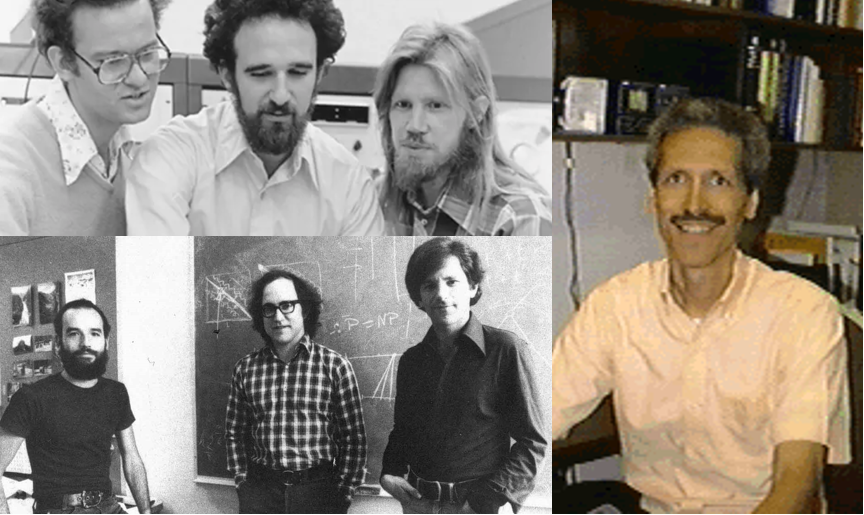
\includegraphics[width=\linewidth, height=1.5in, keepaspectratio]{../figure/rsadhmg.png}
\caption{Top left: Ralph Merkle, Martin Hellman and Whit Diffie, who
together came up in 1976 with the concept of \emph{public key
encryption} and a \emph{key exchange protocol}. Bottom left: Adi Shamir,
Ron Rivest, and Leonard Adleman who, following Diffie and Hellman's
paper, discovered the RSA function that can be used for public key
encryption and digital signatures. Interestingly, one can see the
equation \(\mathbf{P}=\mathbf{NP}\) on the blackboard behind them.
Right: John Gill, who was the first person to suggest to Diffie and
Hellman that they use modular exponentiation as an easy-to-compute but
hard-to-invert function.}
\label{diffiehellmanmerklegillfig}
\end{marginfigure}

\subsection{Defining public key
encryption}\label{Defining-public-key-encry}

A \emph{public key encryption} consists of a triple of algorithms:

\begin{itemize}
\item
  The \emph{key generation algorithm}, which we denote by \(KeyGen\) or
  \(\ensuremath{\mathit{KG}}\) for short, is a randomized algorithm that
  outputs a pair of strings \((e,d)\) where \(e\) is known as the
  \emph{public} (or \emph{encryption}) key, and \(d\) is known as the
  \emph{private} (or \emph{decryption}) key. The key generation
  algorithm gets as input \(1^n\) (i.e., a string of ones of length
  \(n\)). We refer to \(n\) as the \emph{security parameter} of the
  scheme. The bigger we make \(n\), the more secure the encryption will
  be, but also the less efficient it will be.
\item
  The \emph{encryption algorithm}, which we denote by \(E\), takes the
  encryption key \(e\) and a plaintext \(x\), and outputs the ciphertext
  \(y=E_e(x)\).
\item
  The \emph{decryption algorithm}, which we denote by \(D\), takes the
  decryption key \(d\) and a ciphertext \(y\), and outputs the plaintext
  \(x=D_d(y)\).
\end{itemize}


\begin{marginfigure}
\centering
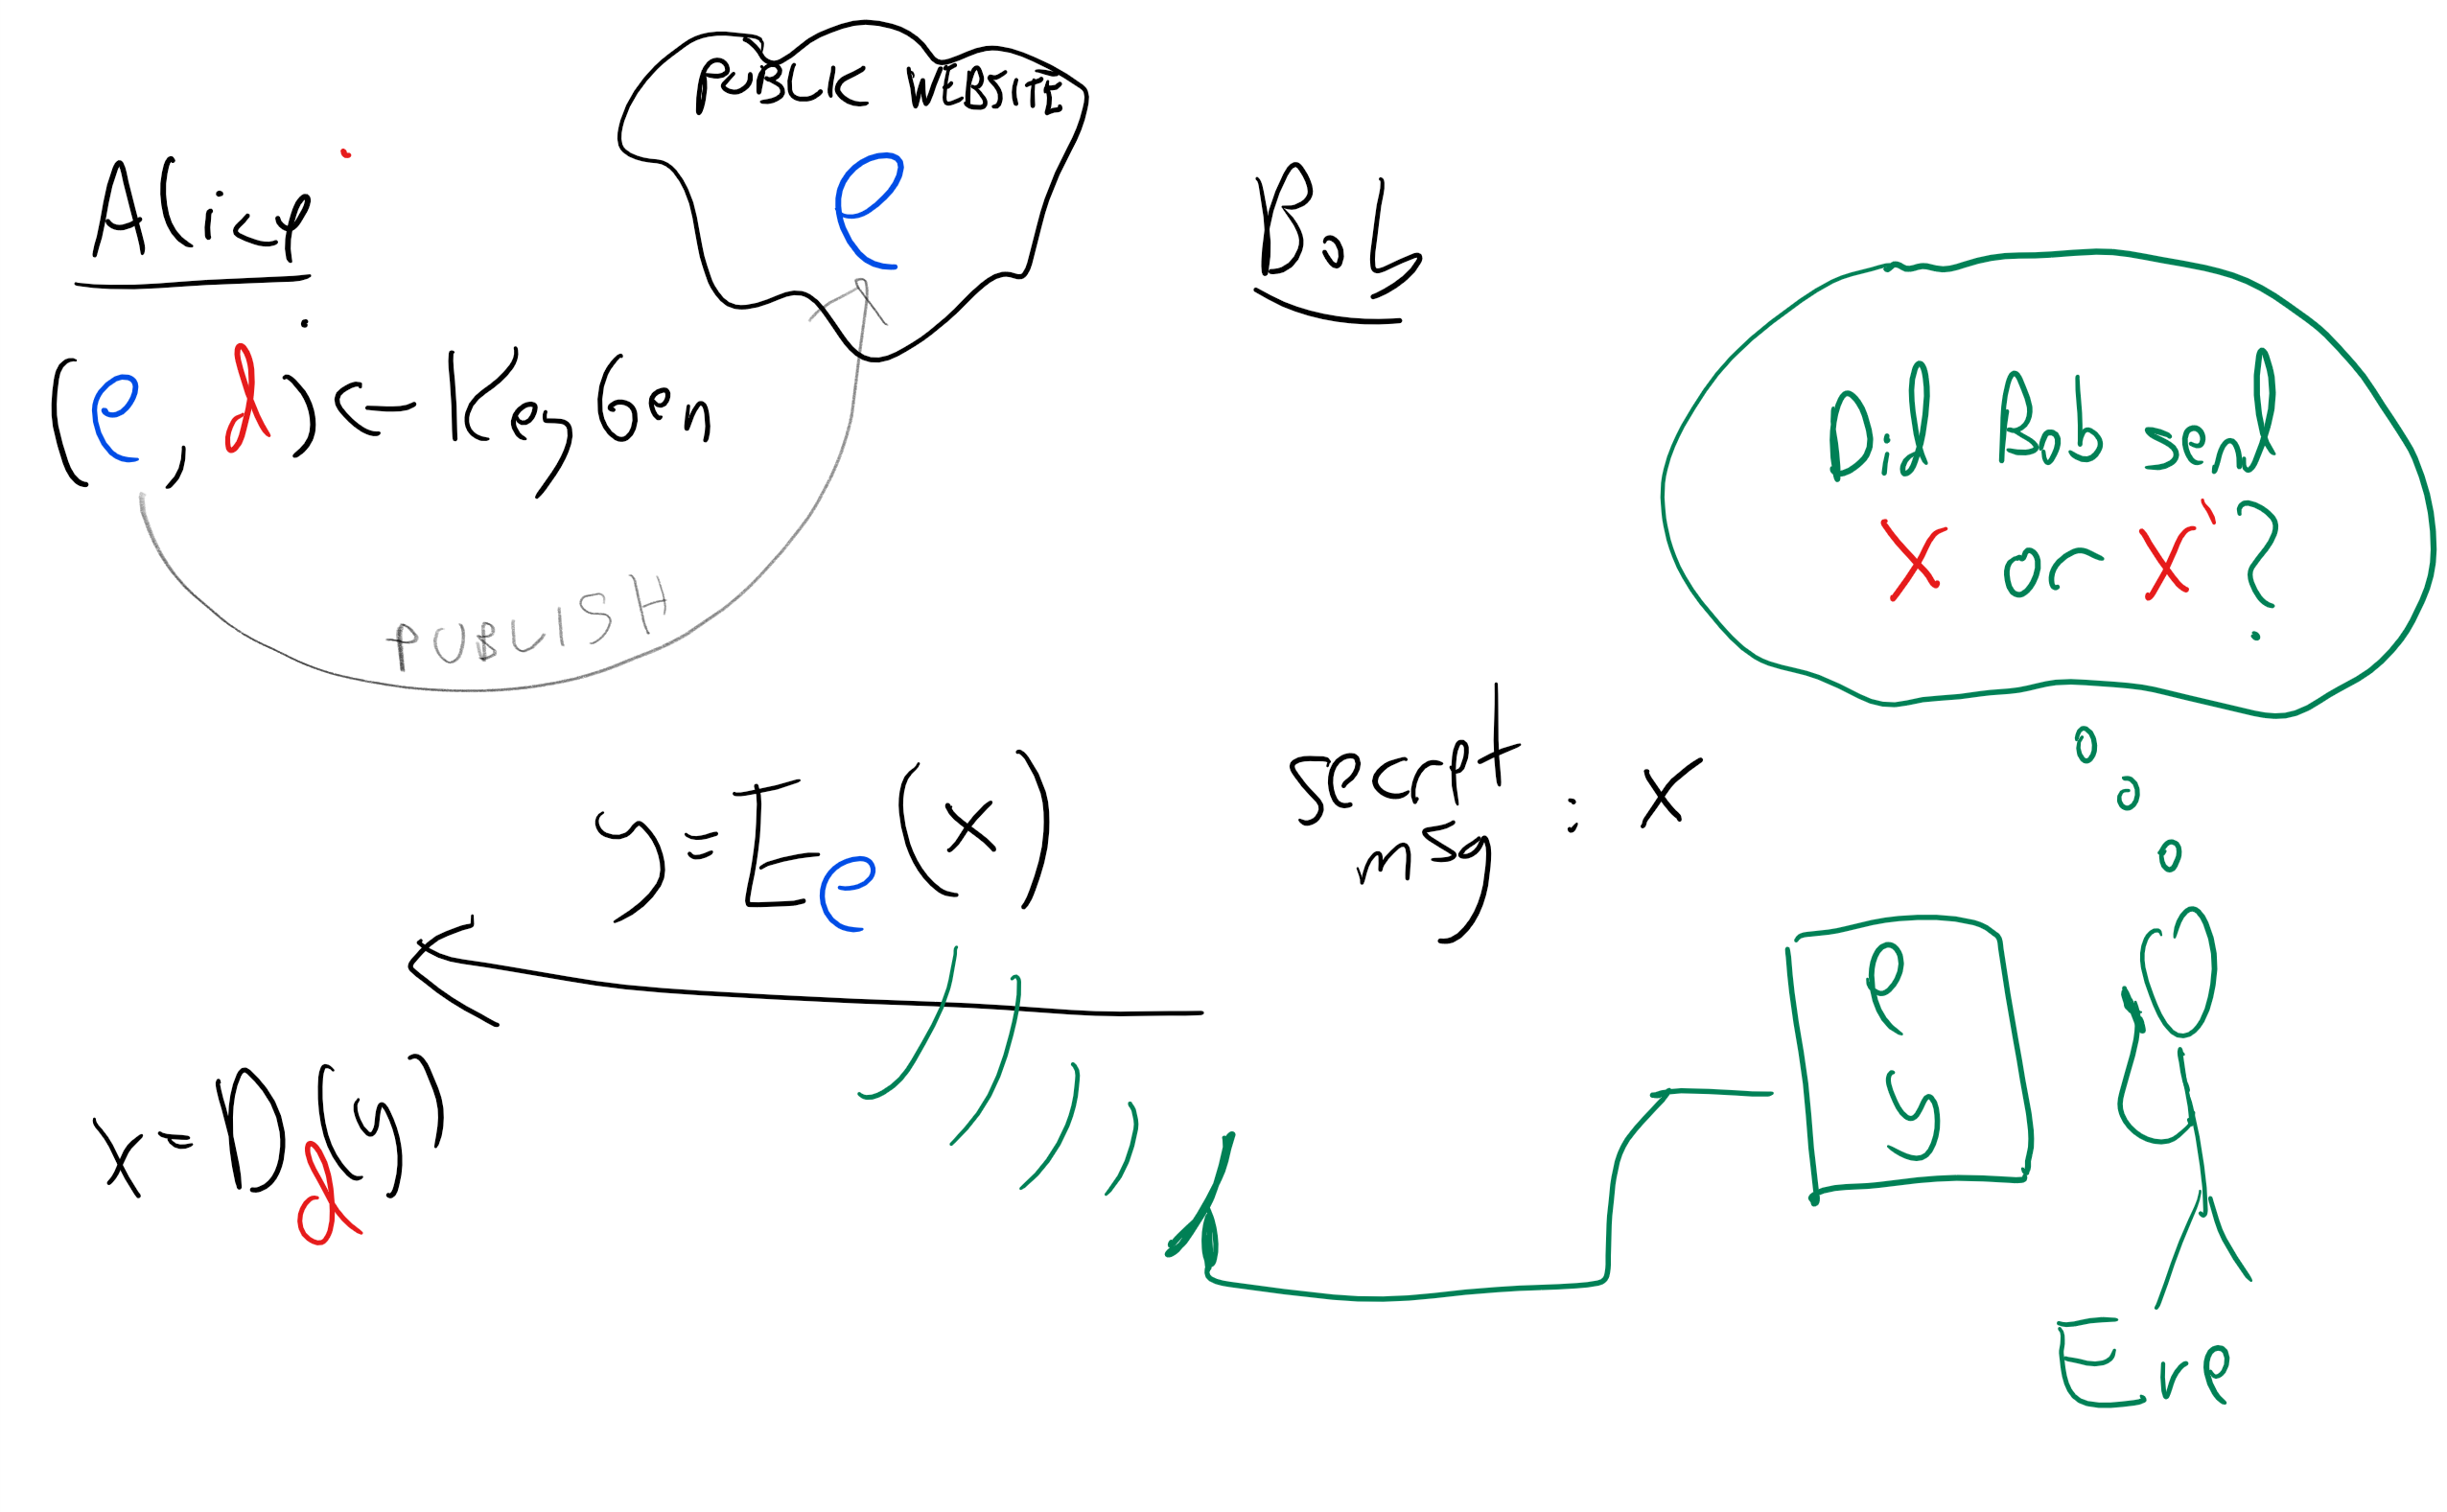
\includegraphics[width=\linewidth, height=1.5in, keepaspectratio]{../figure/publickeyenc.png}
\caption{In a \emph{public key encryption}, Alice generates a
private/public keypair \((e,d)\), publishes \(e\) and keeps \(d\)
secret. To encrypt a message for Alice, one only needs to know \(e\). To
decrypt it we need to know \(d\).}
\label{publickeyencfig}
\end{marginfigure}

We now make this a formal definition:

\hypertarget{publickeyencdef}{}
\begin{definition}[Public Key Encryption] \label[definition]{publickeyencdef}

A \emph{computationally secret public key encryption} with plaintext
length \(L:\N \rightarrow \N\) is a triple of randomized polynomial-time
algorithms \((\ensuremath{\mathit{KG}},E,D)\) that satisfy the following
conditions:

\begin{itemize}
\item
  For every \(n\), if \((e,d)\) is output by
  \(\ensuremath{\mathit{KG}}(1^n)\) with positive probability, and
  \(x\in \{0,1\}^{L(n)}\), then \(D_d(E_e(x))=x\) with probability one.
\item
  For every polynomial \(p\), and sufficiently large \(n\), if \(P\) is
  a NAND-CIRC program of at most \(p(n)\) lines then for every
  \(x,x'\in \{0,1\}^{L(n)}\),
  \(\left| \E[ P(e,E_e(x))] - \E[P(e,E_e(x'))] \right| < 1/p(n)\), where
  this probability is taken over the coins of
  \(\ensuremath{\mathit{KG}}\) and \(E\).
\end{itemize}

\end{definition}

\cref{publickeyencdef} allows \(E\) and \(D\) to be \emph{randomized}
algorithms. In fact, it turns out that it is \emph{necessary} for \(E\)
to be randomized to obtain computational secrecy. It also turns out
that, unlike the private key case, we can transform a public-key
encryption that works for messages that are \emph{only one bit long}
into a public-key encryption scheme that can encrypt arbitrarily long
messages, and in particular messages that are \emph{longer than the
key}. In particular this means that we cannot obtain a perfectly secret
public-key encryption scheme even for one-bit long messages (since it
would imply a perfectly secret public-key, and hence in particular
private-key, encryption with messages longer than the key).

We will not give full constructions for public key encryption schemes in
this chapter, but will mention some of the ideas that underlie the most
widely used schemes today. These generally belong to one of two
families:

\begin{itemize}
\item
  \emph{Group theoretic constructions} based on problems such as
  \emph{integer factoring} and the \emph{discrete logarithm} over finite
  fields or elliptic curves.
\item
  \emph{Lattice/coding based constructions} based on problems such as
  the \emph{closest vector in a lattice} or \emph{bounded distance
  decoding}.
\end{itemize}

Group-theory based encryptions such as the RSA cryptosystem, the
Diffie-Hellman protocol, and Elliptic-Curve Cryptography, are currently
more widely implemented. But the lattice/coding schemes are recently on
the rise, particularly because the known group theoretic encryption
schemes can be broken by \emph{quantum computers}, which we discuss in
\cref{quantumchap}.

\subsection{Diffie-Hellman key
exchange}\label{Diffie-Hellman-key-exchan}

As just one example of how public key encryption schemes are
constructed, let us now describe the Diffie-Hellman key exchange. We
describe the Diffie-Hellman protocol in a somewhat of an informal level,
without presenting a full security analysis.

The computational problem underlying the Diffie Hellman protocol is the
\emph{discrete logarithm problem}. Let's suppose that \(g\) is some
integer. We can compute the map \(x \mapsto g^x\) and also its
\emph{inverse} \(y \mapsto \log_g y\). (For example, we can compute a
logarithm is by \emph{binary search}: start with some interval
\([x_{min},x_{max}]\) that is guaranteed to contain \(\log_g y\). We can
then test whether the interval's midpoint \(x_{mid}\) satisfies
\(g^{x_{mid}} > y\), and based on that halve the size of the interval.)

However, suppose now that we use \emph{modular arithmetic} and work
modulo some prime number \(p\). If \(p\) has \(n\) binary digits and
\(g\) is in \([p]\) then we can compute the map \(x \mapsto g^x \mod p\)
in time polynomial in \(n\). (This is not trivial, and is a great
exercise for you to work this out; as a hint, start by showing that one
can compute the map \(k \mapsto g^{2^k} \mod p\) using \(k\) modular
multiplications modulo \(p\), if you're stumped, you can look up
\href{https://en.wikipedia.org/wiki/Exponentiation_by_squaring}{this
Wikipedia entry}.) On the other hand, because of the ``wraparound''
property of modular arithmetic, we cannot run binary search to find the
inverse of this map (known as the \emph{discrete logarithm}). In fact,
there is no known polynomial-time algorithm for computing this discrete
logarithm map map \((g,x,p) \mapsto \log_g x \mod p\), where we define
\(\log_g x \mod p\) as the number \(a \in [p]\) such that
\(g^a = x \mod p\).

The Diffie-Hellman protocol for Bob to send a message to Alice is as
follows:

\begin{itemize}
\item
  \textbf{Alice:} Chooses \(p\) to be a random \(n\) bit long prime
  (which can be done by choosing random numbers and running a primality
  testing algorithm on them), and \(g\) and \(a\) at random in \([p]\).
  She sends to Bob the triple \((p,g,g^a \mod p)\).
\item
  \textbf{Bob:} Given the triple \((p,g,h)\), Bob sends a message
  \(x \in \{0,1\}^L\) to Alice by choosing \(b\) at random in \([p]\),
  and sending to Alice the pair
  \((g^b \mod p, rep(h^b \mod p) \oplus x)\) where
  \(rep:[p] \rightarrow \{0,1\}^*\) is some ``representation function''
  that maps \([p]\) to \(\{0,1\}^L\). (The function \(rep\) does not
  need to be one-to-one and you can think of \(rep(z)\) as simply
  outputting \(L\) of the bits of \(z\) in the natural binary
  representation, it does need to satisfy certain technical conditions
  which we omit in this description.)
\item
  \textbf{Alice:} Given \(g',z\), Alice recovers \(x\) by outputting
  \(rep(g'^a \mod p) \oplus z\).
\end{itemize}

The correctness of the protocol follows from the simple fact that
\((g^a)^b = (g^b)^a\) for every \(g,a,b\) and this still holds if we
work modulo \(p\). Its security relies on the computational assumption
that computing this map is hard, even in a certain ``average case''
sense (this computational assumption is known as the
\href{https://en.wikipedia.org/wiki/Decisional_Diffie\%E2\%80\%93Hellman_assumption}{Decisional
Diffie Hellman assumption}). The Diffie-Hellman key exchange protocol
can be thought of as a public key encryption where the Alice's first
message is the public key, and Bob's message is the encryption.

One can think of the Diffie-Hellman protocol as being based on a
``trapdoor pseudorandom generator'' whereas the triple
\(g^a,g^{b},g^{ab}\) looks ``random'' to someone that doesn't know
\(a\), but someone that does know \(a\) can see that raising the second
element to the \(a\)-th power yields the third element. The
Diffie-Hellman protocol can be described abstractly in the context of
any \href{https://en.wikipedia.org/wiki/Abelian_group}{finite Abelian
group} for which we can efficiently compute the group operation. It has
been implemented on other groups than numbers modulo \(p\), and in
particular
\href{https://en.wikipedia.org/wiki/Elliptic-curve_cryptography}{Elliptic
Curve Cryptography (ECC)} is obtained by basing the Diffie Hellman on
elliptic curve groups which gives some practical advantages. Another
common group theoretic basis for key-exchange/public key encryption
protocol is the RSA function. A big disadvantage of Diffie-Hellman (both
the modular arithmetic and elliptic curve variants) and RSA is that both
schemes can be broken in polynomial time by a \emph{quantum computer}.
We will discuss quantum computing later in this course.

\section{Other security notions}\label{Other-security-notions}

There is a great deal to cryptography beyond just encryption schemes,
and beyond the notion of a passive adversary. A central objective is
\emph{integrity} or \emph{authentication}: protecting communications
from being modified by an adversary. Integrity is often more fundamental
than secrecy: whether it is a software update or viewing the news, you
might often not care about the communication being secret as much as
that it indeed came from its claimed source. \emph{Digital signature
schemes} are the analog of public key encryption for authentication, and
are widely used (in particular as the basis for
\href{https://en.wikipedia.org/wiki/Public_key_certificate}{public key
certificates}) to provide a foundation of trust in the digital world.

Similarly, even for encryption, we often need to ensure security against
\emph{active attacks}, and so notions such as non-malleability and
\href{https://en.wikipedia.org/wiki/Adaptive_chosen-ciphertext_attack}{adaptive
chosen ciphertext} security have been proposed. An encryption scheme is
only as secure as the secret key, and mechanisms to make sure the key is
generated properly, and is protected against refresh or even compromise
(i.e., \href{https://en.wikipedia.org/wiki/Forward_secrecy}{forward
secrecy}) have been studied as well. Hopefully this chapter provides you
with some appreciation for cryptography as an intellectual field, but
does not imbue you with a false self of confidence in implementing it.

\emph{Cryptographic hash functions} is another widely used tool with a
variety of uses, including extracting randomness from high entropy
sources, achieving hard-to-forge short ``digests'' of files, protecting
passwords, and much more.

\section{Magic}\label{Magic}

Beyond encryption and signature schemes, cryptographers have managed to
obtain objects that truly seem paradoxical and ``magical''. We briefly
discuss some of these objects. We do not give any details, but hopefully
this will spark your curiosity to find out more.

\subsection{Zero knowledge proofs}\label{Zero-knowledge-proofs}

On October 31, 1903, the mathematician Frank Nelson Cole, gave an
hourlong lecture to a meeting of the American Mathematical Society where
he did not speak a single word. Rather, he calculated on the board the
value \(2^{67}-1\) which is equal to \(147,573,952,589,676,412,927\),
and then showed that this number is equal to
\(193,707,721 \times 761,838,257,287\). Cole's proof showed that
\(2^{67}-1\) is not a prime, but it also revealed additional
information, namely its actual factors. This is often the case with
proofs: they teach us more than just the validity of the statements.

In \emph{Zero Knowledge Proofs} we try to achieve the opposite effect.
We want a proof for a statement \(X\) where we can \emph{rigorously
show} that the proofs reveals \emph{absolutely no additional information
about \(X\)} beyond the fact that it is true. This turns out to be an
extremely useful object for a variety of tasks including authentication,
secure protocols, voting,
\href{https://z.cash/technology/zksnarks.html}{anonymity in
cryptocurrencies}, and more. Constructing these objects relies on the
theory of \(\mathbf{NP}\) completeness. Thus this theory that originally
was designed to give a \emph{negative result} (show that some problems
are hard) ended up yielding \emph{positive applications}, enabling us to
achieve tasks that were not possible otherwise.

\subsection{Fully homomorphic
encryption}\label{Fully-homomorphic-encrypt}

Suppose that we are given a bit-by-bit encryption of a string
\(E_k(x_0),\ldots,E_k(x_{n-1})\). By design, these ciphertexts are
supposed to be ``completely unscrutable'' and we should not be able to
extract any information about \(x_i\)'s from it. However, already in
1978, Rivest, Adleman and Dertouzos observed that this does not imply
that we could not \emph{manipulate} these encryptions. For example, it
turns out the security of an encryption scheme does not immediately rule
out the ability to take a pair of encryptions \(E_k(a)\) and \(E_k(b)\)
and compute from them \(E_k(a \ensuremath{\mathit{NAND}} b)\)
\emph{without knowing the secret key \(k\)}. But do there exist
encryption schemes that allow such manipulations? And if so, is this a
bug or a feature?

Rivest et al already showed that such encryption schemes could be
\emph{immensely} useful, and their utility has only grown in the age of
cloud computing. After all, if we can compute NAND then we can use this
to run any algorithm \(P\) on the encrypted data, and map
\(E_k(x_0),\ldots,E_k(x_{n-1})\) to \(E_k(P(x_0,\ldots,x_{n-1}))\). For
example, a client could store their secret data \(x\) in encrypted form
on the cloud, and have the cloud provider perform all sorts of
computation on these data without ever revealing to the provider the
private key, and so without the provider \emph{ever learning any
information} about the secret data.

The question of \emph{existence} of such a scheme took much longer time
to resolve. Only in 2009 Craig Gentry gave the first construction of an
encryption scheme that allows to compute a universal basis of gates on
the data (known as a \emph{Fully Homomorphic Encryption scheme} in
crypto parlance). Gentry's scheme left much to be desired in terms of
efficiency, and improving upon it has been the focus of an intensive
research program that has already seen significant improvements.

\subsection{Multiparty secure
computation}\label{Multiparty-secure-computa}

Cryptography is about enabling mutually distrusting parties to achieve a
common goal. Perhaps the most general primitive achieving this objective
is
\href{https://en.wikipedia.org/wiki/Secure_multi-party_computation}{secure
multiparty computation}. The idea in secure multiparty computation is
that \(n\) parties interact together to compute some function
\(F(x_0,\ldots,x_{n-1})\) where \(x_i\) is the private input of the
\(i\)-th party. The crucial point is that there is \emph{no commonly
trusted party or authority} and that nothing is revealed about the
secret data beyond the function's output. One example is an
\emph{electronic voting protocol} where only the total vote count is
revealed, with the privacy of the individual voters protected, but
without having to trust any authority to either count the votes
correctly or to keep information confidential. Another example is
implementing a
\href{https://en.wikipedia.org/wiki/Vickrey_auction}{second price (aka
Vickrey) auction} where \(n-1\) parties submit bids to an item owned by
the \(n\)-th party, and the item goes to the highest bidder but at the
price of the \emph{second highest bid}. Using secure multiparty
computation we can implement second price auction in a way that will
ensure the secrecy of the numerical values of all bids (including even
the top one) except the second highest one, and the secrecy of the
identity of all bidders (including even the second highest bidder)
except the top one. We emphasize that such a protocol requires no trust
even in the auctioneer itself, that will also not learn any additional
information. Secure multiparty computation can be used even for
computing \emph{randomized} processes, with one example being playing
Poker over the net without having to trust any server for correct
shuffling of cards or not revealing the information.

\begin{recap} \label[recap]{We-can-formally-define-th}

\begin{itemize}
\item
  We can formally define the notion of security of an encryption scheme.
\item
  \emph{Perfect secrecy} ensures that an adversary does not learn
  \emph{anything} about the plaintext from the ciphertext, regardless of
  their computational powers.
\item
  The one-time pad is a perfectly secret encryption with the length of
  the key equaling the length of the message. No perfectly secret
  encryption can have key shorter than the message.
\item
  \emph{Computational secrecy} can be as good as perfect secrecy since
  it ensures that the advantage that computationally bounded adversaries
  gain from observing the ciphertext is exponentially small. If the
  optimal PRG conjecture is true then there exists a computationally
  secret encryption scheme with messages that can be (almost)
  \emph{exponentially bigger} than the key.
\item
  There are many cryptographic tools that go well beyond private key
  encryption. These include \emph{public key encryption}, \emph{digital
  signatures} and \emph{hash functions}, as well as more ``magical''
  tools such as \emph{multiparty secure computation}, \emph{fully
  homomorphic encryption}, \emph{zero knowledge proofs}, and many
  others.
\end{itemize}

\end{recap}

\section{Exercises}\label{Exercises}

\section{Bibliographical notes}\label{Bibliographical-notes}

Much of this text is taken from \href{https://intensecrypto.org}{my
lecture notes on cryptography}.

Shannon's manuscript was written in 1945 but was classified, and a
partial version was only published in 1949. Still it has revolutionized
cryptography, and is the forerunner to much of what followed.

The Venona project's history is described in
\href{http://nsarchive.gwu.edu/NSAEBB/NSAEBB278/01.PDF}{this document}.
Aside from Grabeel and Zubko, credit to the discovery that the Soviets
were reusing keys is shared by Lt. Richard Hallock, Carrie Berry, Frank
Lewis, and Lt. Karl Elmquist, and there are others that have made
important contribution to this project. See pages 27 and 28 in the
document.

In a
\href{https://www.nsa.gov/news-features/declassified-documents/nash-letters/assets/files/nash_letters1.pdf}{1955
letter to the NSA} that only recently came forward, John Nash proposed
an ``unbreakable'' encryption scheme. He wrote \emph{``I hope my
handwriting, etc. do not give the impression I am just a crank or
circle-squarer\ldots. The significance of this conjecture {[}that
certain encryption schemes are exponentially secure against key recovery
attacks{]} .. is that it is quite feasible to design ciphers that are
effectively unbreakable.''}. John Nash made seminal contributions in
mathematics and game theory, and was awarded both the Abel Prize in
mathematics and the Nobel Memorial Prize in Economic Sciences. However,
he has struggled with mental illness throughout his life. His biography,
\href{https://en.wikipedia.org/wiki/A_Beautiful_Mind_(book)}{A Beautiful
Mind} was made into a popular movie. It is natural to compare Nash's
1955 letter to the NSA to Gödel's letter to von Neumann we mentioned
before. From the theoretical computer science point of view, the crucial
difference is that while Nash informally talks about exponential vs
polynomial computation time, he does not mention the word ``Turing
Machine'' or other models of computation, and it is not clear if he is
aware or not that his conjecture can be made mathematically precise
(assuming a formalization of ``sufficiently complex types of
enciphering'').

The definition of computational secrecy we use is the notion of
\emph{computational indistinguishability} (known to be equivalent to
\emph{semantic security}) that was given by Goldwasser and Micali in
1982.

Although they used a different terminology, Diffie and Hellman already
made clear in their paper that their protocol can be used as a public
key encryption, with the first message being put in a ``public file''.
In 1985, ElGamal showed how to obtain a \emph{signature scheme} based on
the Diffie Hellman ideas, and since he described the Diffie-Hellman
encryption scheme in the same paper, the public key encryption scheme
originally proposed by Diffie and Hellman is sometimes also known as
ElGamal encryption.

\href{https://eccc.weizmann.ac.il/report/2017/065/}{My survey} contains
a discussion on the different types of public key assumptions. While the
standard elliptic curve cryptographic schemes are as susceptible to
quantum computers as Diffie-Hellman and RSA, their main advantage is
that the best known classical algorithms for computing discrete
logarithms over elliptic curve groups take time \(2^{\epsilon n}\) for
some \(\epsilon>0\) where \(n\) is the number of bits to describe a
group element. In contrast, for the multiplicative group modulo a prime
\(p\) the best algorithm take time \(2^{O(n^{1/3} polylog(n))}\) which
means that (assuming the known algorithms are optimal) we need to set
the prime to be bigger (and so have larger key sizes with corresponding
overhead in communication and computation) to get the same level of
security.

Zero-knowledge proofs were constructed by Goldwasser, Micali, and
Rackoff in 1982, and their wide applicability was shown (using the
theory of \(\mathbf{NP}\) completeness) by Goldreich, Micali, and
Wigderson in 1986.

Two party and multiparty secure computation protocols were constructed
(respectively) by Yao in 1982 and Goldreich, Micali, and Wigderson in
1987. The latter work gave a general transformation from security
against passive adversaries to security against active adversaries using
zero knowledge proofs.
